\documentclass{../lab}

\labacronym{QIE}
\labtitle{Quantum Interference \& Entanglement}

%\newcommand{\[1]}{http://advancedlab.berkeley.edu/mediawiki/index.php/Quantum_Interference_\%26_Entanglement#cite_note-Dehlinger-0}
%\newcommand{\[3]}{http://advancedlab.berkeley.edu/mediawiki/index.php/Quantum_Interference_\%26_Entanglement#cite_note-CHSH-2}

\begin{document}

\maketitle

\tableofcontents

\section{Quantum Interference \& Entanglement Description (QIE)}

\begin{itemize}
    \item Pre-requisites: Physics 137A

    \item Days Allotted for the Experiment: 6

\end{itemize}

\textbf{Attention: There is NO eating or drinking in the 111-Lab anywhere, except in rooms 282 \& 286 LeConte on the bench with the BLUE stripe around it.} Thank You, the Staff.

This lab will be graded 30\% on theory, 40\% on technique, and 30\% on analysis. For more information, see the \href{http://experimentationlab.berkeley.edu/syllabus}{\textbf{Advanced Lab Syllabus}}.

Comments: E-mail \href{\MailDonOrlando}{\textbf{Don Orlando}}

\section{Quantum Interference \& Entanglement Pictures}

\noindent
\begin{figure}[!htb]
\minipage{0.32\linewidth}
  \href{http://experimentationlab.berkeley.edu/sites/default/files/images/QIE_0613_Crop_.jpg}{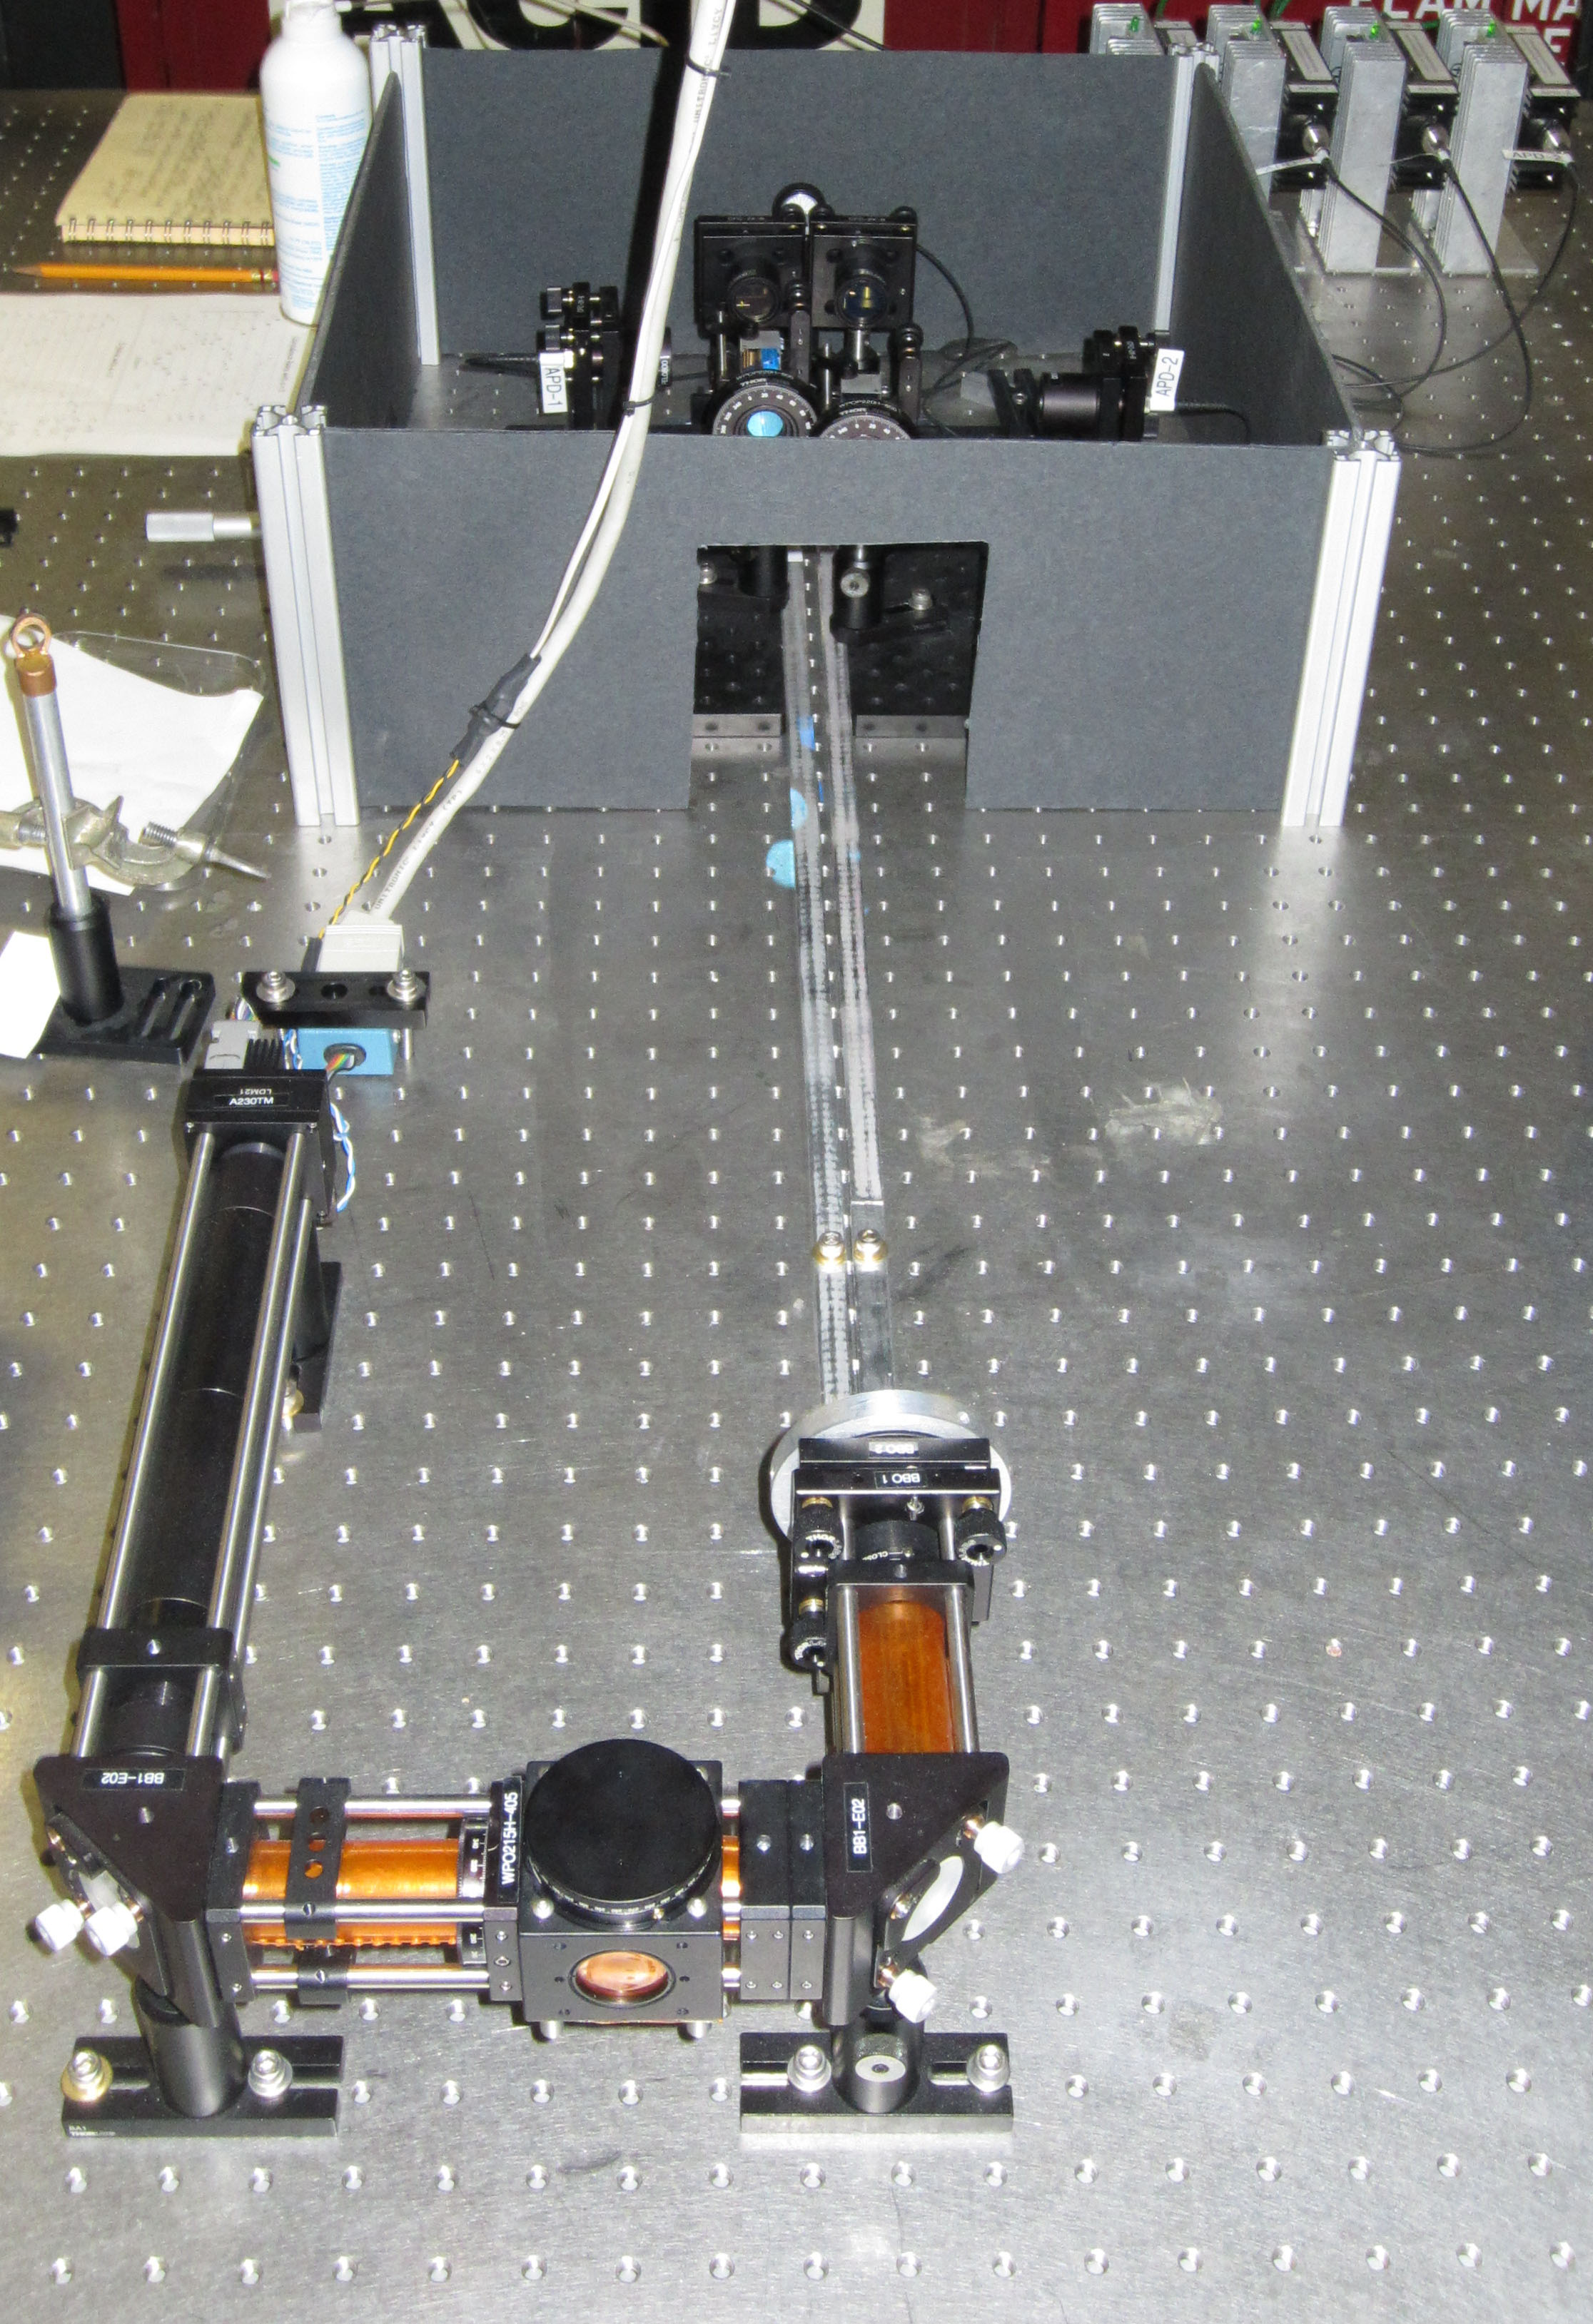
\includegraphics[width=\linewidth,keepaspectratio]{images/QIE_0613_Crop_.jpg}}
  \caption{Quantum Interference \& Entanglement Experiment \\ \href{http://experimentationlab.berkeley.edu/sites/default/files/images/QIE_0613_Crop_.jpg}{Click here to see larger picture}}
  \label{fig:Apparatus}
\endminipage\hfill
\minipage{0.32\linewidth}
  \href{http://experimentationlab.berkeley.edu/sites/default/files/images/QIE_0615.jpg}{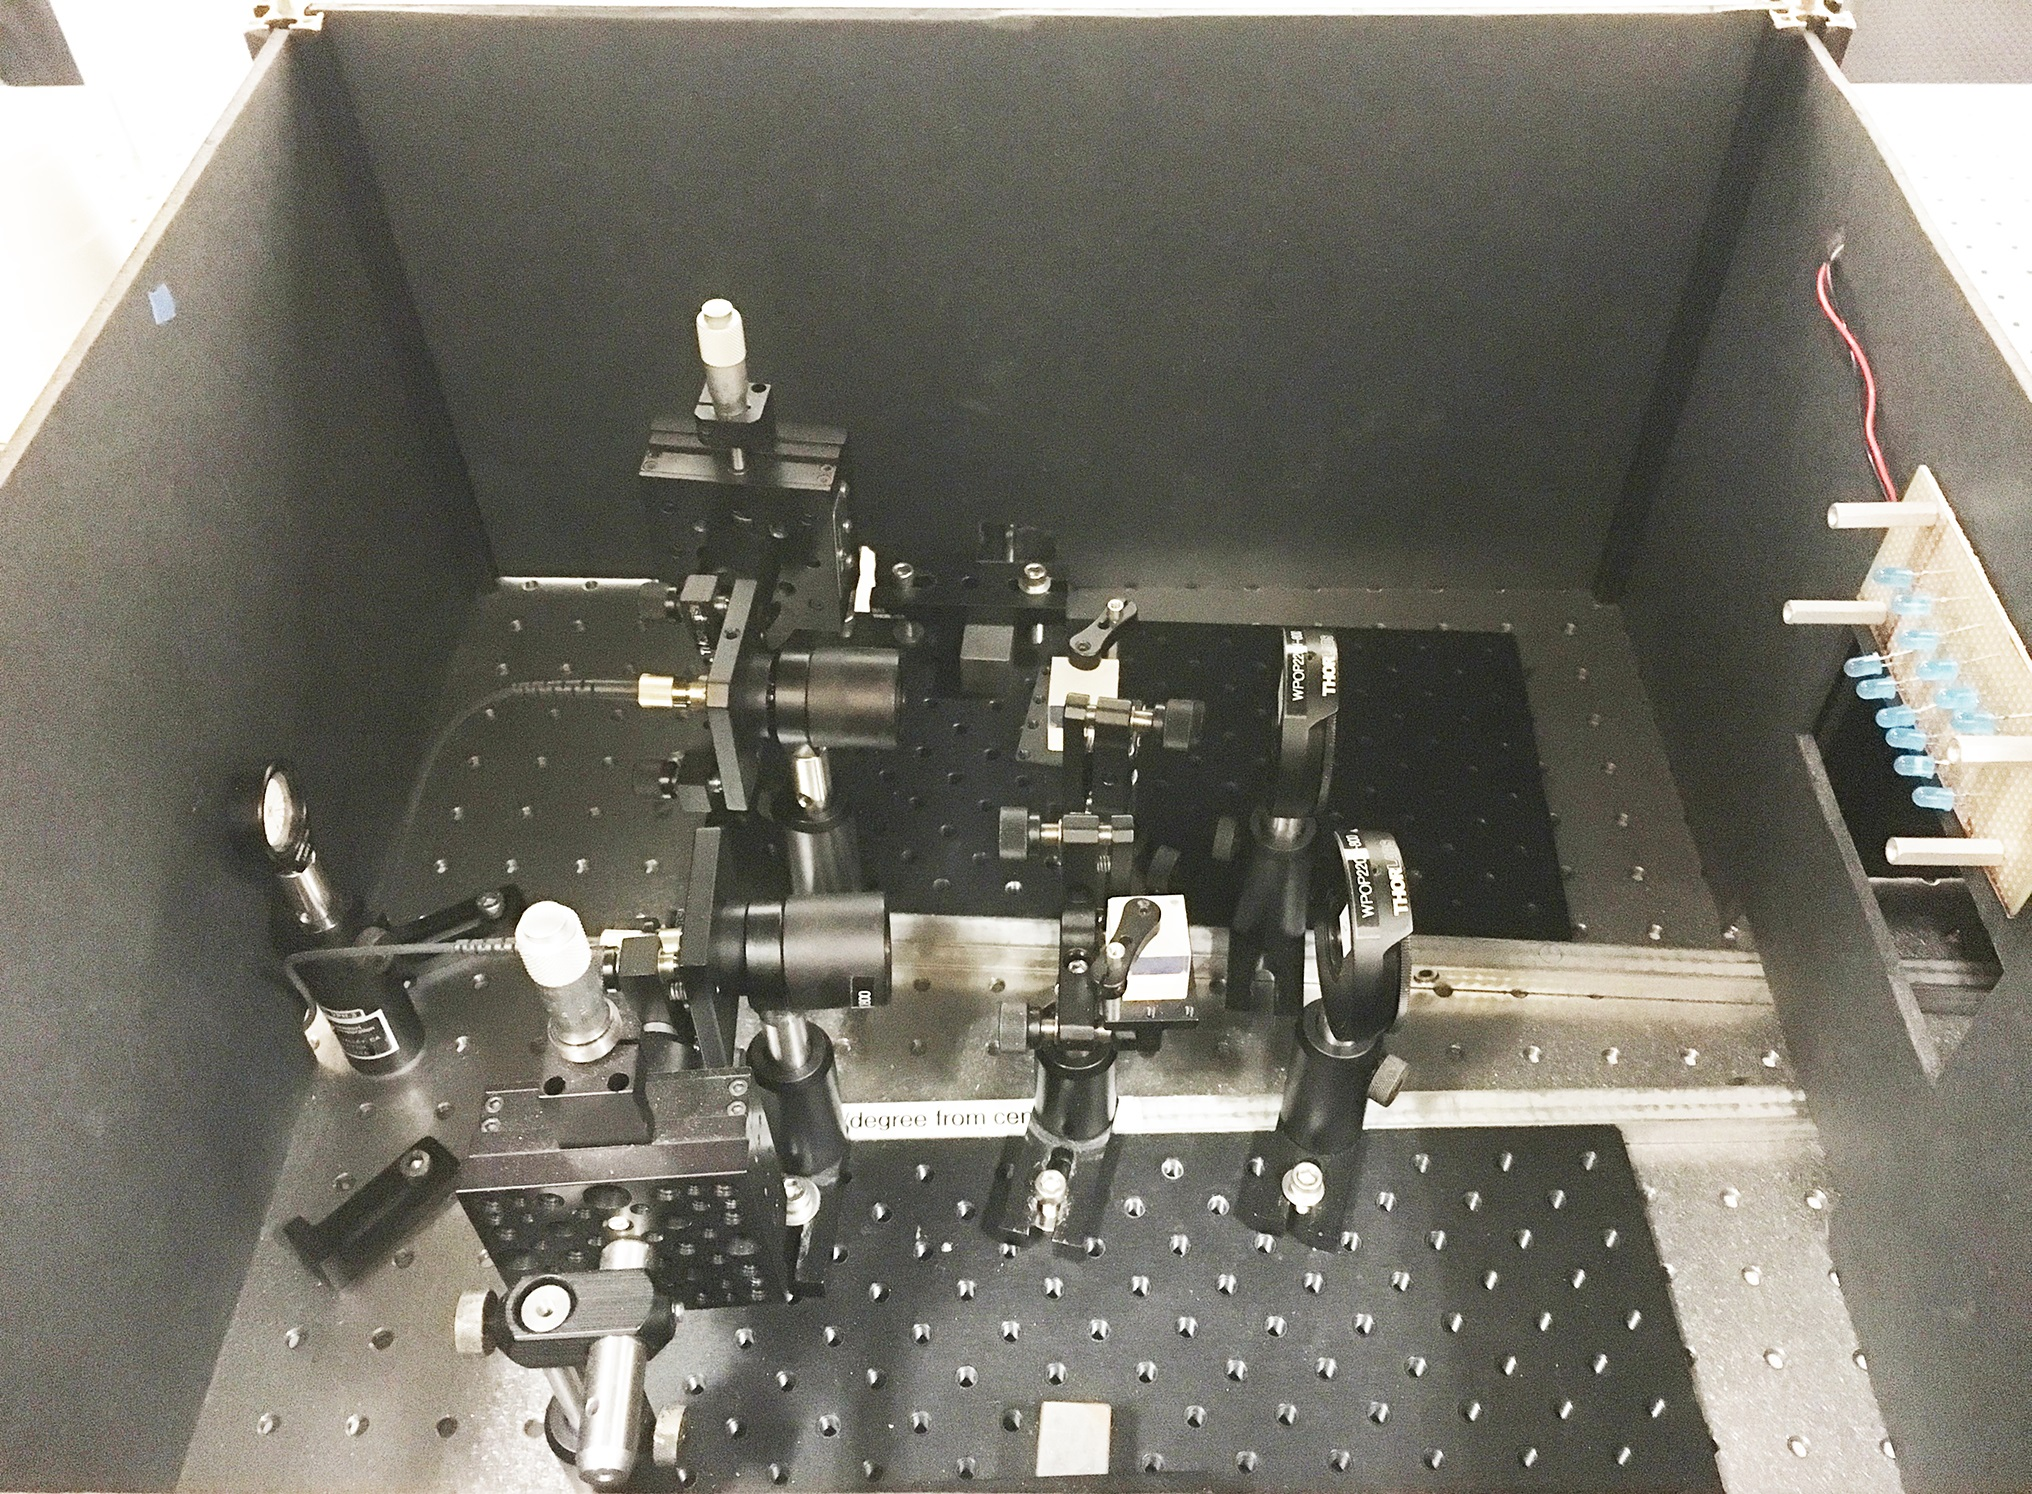
\includegraphics[width=\linewidth,keepaspectratio]{images/QIE_0615.jpg}}
  \caption{Lead Pig where source is placed \\
  \href{http://experimentationlab.berkeley.edu/sites/default/files/images/GMA_Pig_3536-Lg.jpg}{Click here to see larger picture}}
  \label{fig:LeadPig}
\endminipage\hfill
\minipage{0.32\linewidth}
  \href{http://experimentationlab.berkeley.edu/sites/default/files/images/GMA_Layout_3537-Lg.jpg}{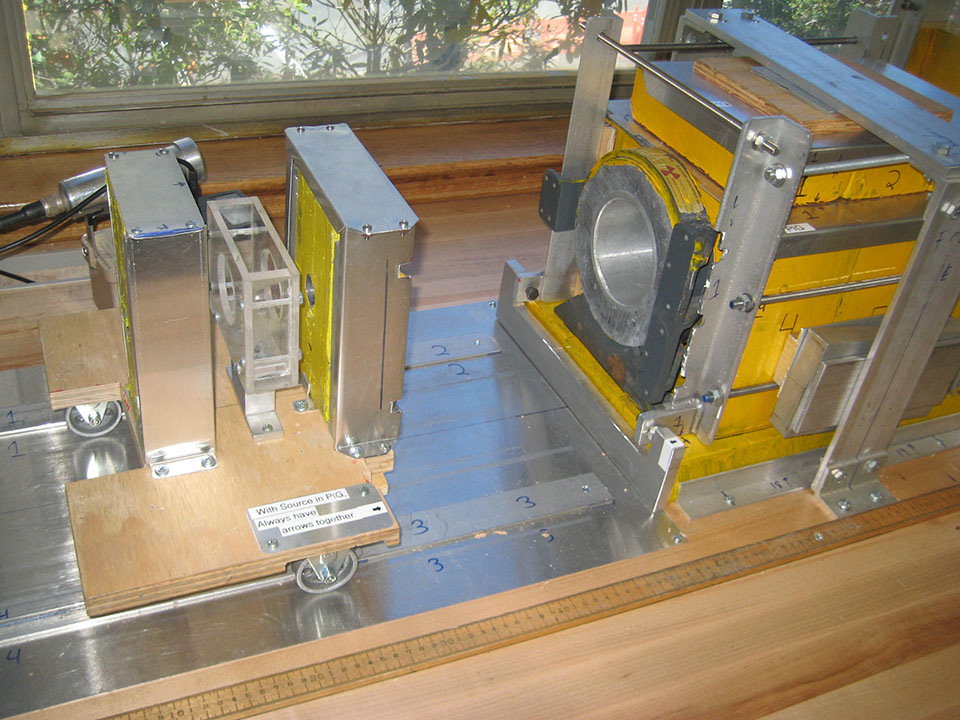
\includegraphics[width=\linewidth,keepaspectratio]{images/GMA_Layout_3537-Lg.jpg}}
  \caption{Pig \& Collimator where source is placed \\ \href{http://experimentationlab.berkeley.edu/sites/default/files/images/GMA_Layout_3537-Lg.jpg}{Click here to see larger picture}}\label{fig:PigCollimator}
\endminipage
\end{figure}



\href{http://experimentationlab.berkeley.edu/sites/default/files/images/QIE_APDs_0616.jpg}{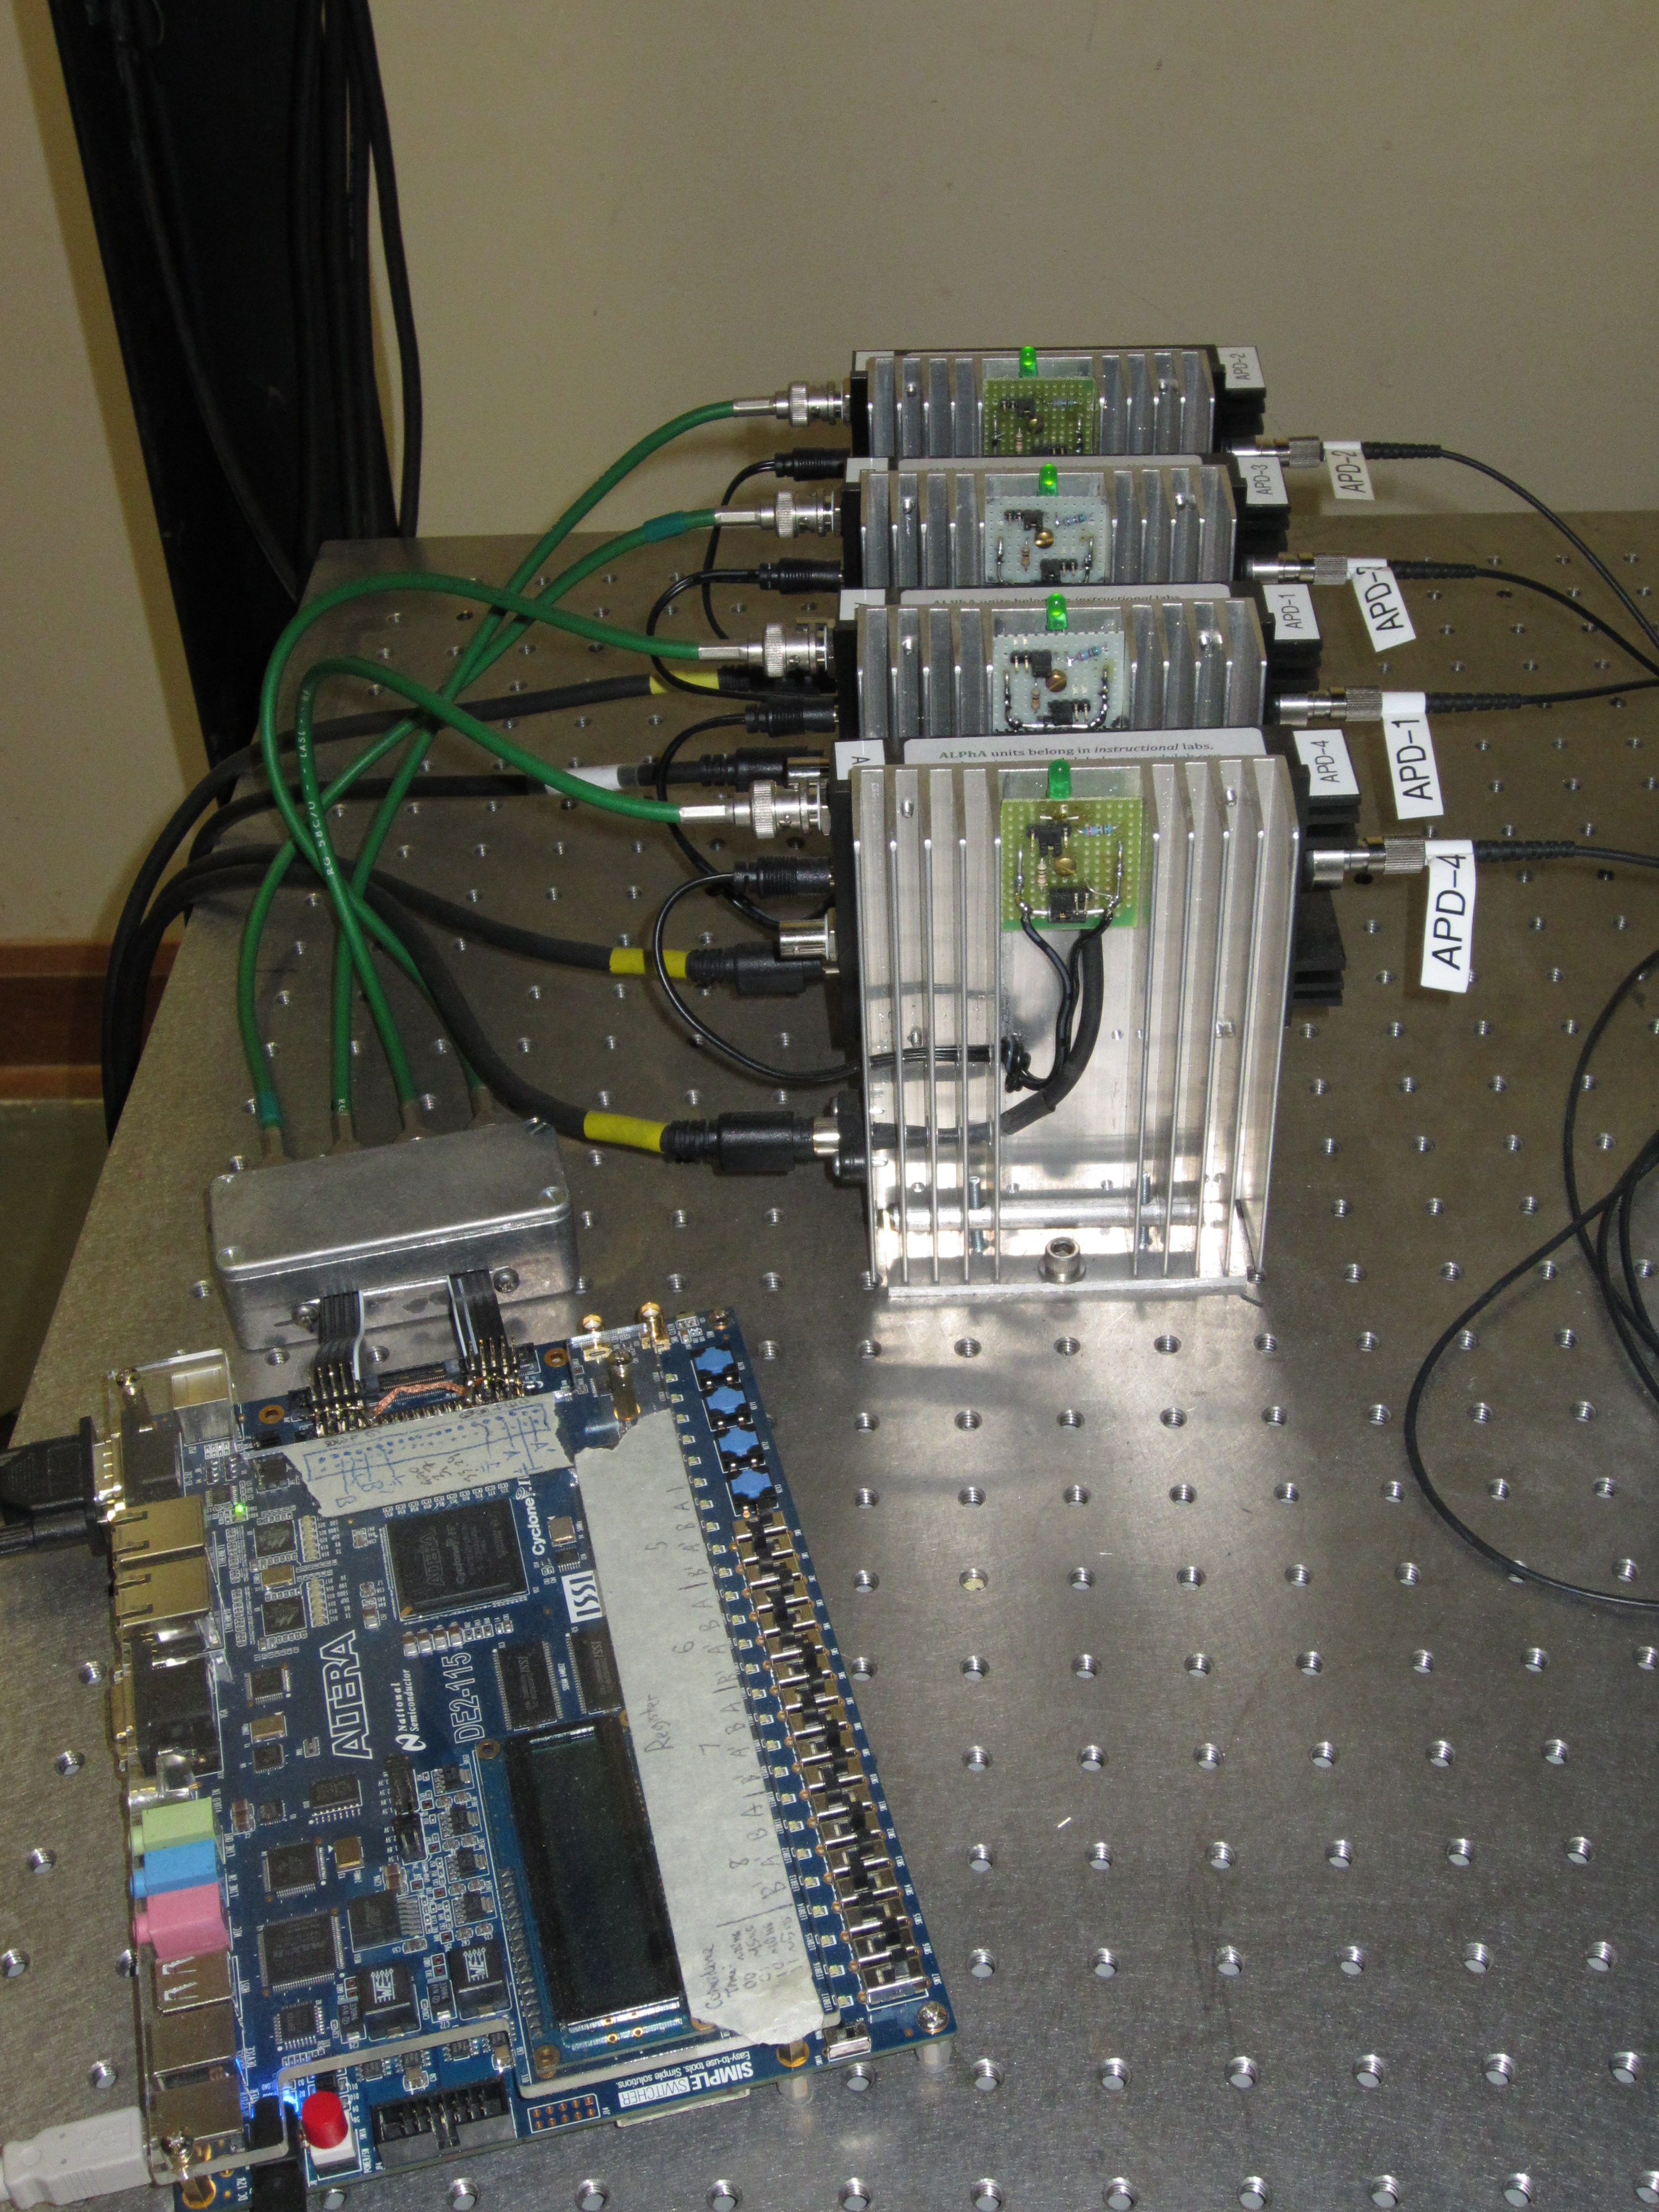
\includegraphics[width=0.33\linewidth,keepaspectratio]{images/QIE_APDs_0616.jpg}}

\section{Before the 1st Day of Lab}

\textbf{Complete the following before your experiment's scheduled start date:}

\begin{enumerate}
    \item View the\textbf{ }\href{http://experimentationlab.berkeley.edu/sites/default/files/QIE/qie\_introduction\_final2.mp4}{\textbf{introduction video}} or this experiment. Read the references \cite{Dehlinger}, \cite{Bell}, \cite{Clauser} below. \cite{Dehlinger} is particularly useful.

    \item Check points are examination points that are placed in this lab where you must STOP and call a GSI or professor to make sure you understand what's expected. There could  be multiple check points throughout your lab so make sure you don't skip them since there is a \emph{\href{http://experimentationlab.berkeley.edu/qiecheckpoints}{\textbf{sign off sheet}}} that must be turned in with your lab report. There are 5 Checkpoints in this lab.

    \item Read the \href{http://experimentationlab.berkeley.edu/sites/default/files/QIE/fundamental-Optics.pdf}{\textbf{Optics Tutorial}}, in particular sections 1.41 (Polarization), 1.46 (Waveplates, and 1.55 (Beamsplitter Cubes). You should also look at Optical Coatings (all of our waveplates have antireflection coatings), and Intro to Laser Technology. You will not get very far if you do not understand how these optics work, it will be essential to prepare before you start working on the lab.

    \item Complete the training for the safe use of lasers detailed on the \href{http://experimentationlab.berkeley.edu/lasersafety}{\textbf{\textbf{Laser Safety Training}}} page. This includes readings, watching a video, taking a quiz, and filling out a form.

    \item Print, fill out the Pre-Lab, Mid-Lab and QIE Evaluation \href{http://experimentationlab.berkeley.edu/qieprelab}{\textbf{QIE Pre Lab and Evaluation}}. The pre-lab must be printed separately and turn in your answers with the signed PreLab. Discuss the experiment and pre-lab questions with any faculty member or GSI and get it signed off by that faculty member or GSI. Turn in the signed Pre-lab, Mid-Lab, and QIE Evaluation sheet with your lab report.

    \item Last day of the experiment please fill out the MOT  \href{\ExperimentEvaluation}{\textbf{Experiment Evaluation}}

\end{enumerate}

You should keep a laboratory notebook. The notebook should contain a detailed record of everything that was done and how/why it was done, as well as all of the data and analysis, also with plenty of how/why entries. This will aid you when you write your report.

Other References [\href{http://physics111.lib.berkeley.edu/Physics111/Reprints/QIE/QIE\_index.html}{\textbf{Physics 111 Library Site}}]

\section{Objectives}

\begin{itemize}
    \item Learn and experience quantum mechanics and in particular entanglement

    \item Learn to handle and align optics (Half-Wave plates, Polarized Beam Splitters, etc...)

    \item Learn about coincidence techniques

    \item Learn how to violate Bell's Inequality

\end{itemize}

\section{Introduction}
\label{sec:Introduction}

This experiment tests the validity of quantum mechanics against local hidden variable theories in describing entanglement phenomena. It takes the form of a quantum optics experiment using polarization-entangled photon pairs.

\subsection{Bell's Theorem and the CHSH Inequality}

John Bell showed that any theory in which properties are local and are well-defined prior to measurement must obey certain limitations. Interestingly, quantum mechanics exceeds those limits set by these so-called Bell-inequalities. Therefore, observing that nature does exceed these limits makes a good case for quantum mechanics and proves that there exists no local realistic theory that can describe nature accurately. One particular version of the Bell's theorem is the so-called CHSH inequality (named after Clauser, Horne, Shimony, and Holt). To make the discussion more concrete, we will assume a photon source that sends two photons one to each of two distant locations. The degree-of-freedom we will study is the polarization of these photons. We will be interested only in events where the polarization of both photons has been detected successfully. First let us define the \emph{parity} of the polarization correlations:
\begin{equation}
    E = \frac{N_{vv}-N_{vh}-N_{hv}+N_{hh}}{N_\text{total}} = \frac{N_{vv} - N_{vh} - N_{hv} + N_{hh}}{N_{vv} + N_{vh} + N_{hv} + N_{hh}},
\end{equation}
where $N_{vv}$ is the number (or rate) of coincidences where both photons are vertically polarized, etc. $E$ can range from -1, meaning that all photon coincidences have opposite polarizations, to 1, meaning they all have the same polarization. Let us then define the quantity, $S$, which is function of four distinct $E$ measurements.
\begin{equation}
    S=E(\alpha,\beta)-E(\alpha,\beta') + E(\alpha',\beta) + E(\alpha',\beta') \,,
\end{equation}
where $\alpha$ and $\beta$ are the angles in which we are going to analyze the polarization of each photon. The interest of defining the quantity $S$ is that local realistic theories are always bound to yield $|S| \leq 2$, while quantum mechanics allows values of up to $2\sqrt{2} \approx 2.8$.

At first glance, it would seem that $S$ could range from –4 to 4. However, a careful inspection of the physics reveals that no two pairs of angles ($\alpha,\alpha'$) and ($\beta,\beta'$) give a value this large. If the system obeys a local hidden variable theory, then $S$ is restricted by the CHSH inequality: $|S| \leq 2$. However, quantum mechanics predicts that $|S|$ can be as high as 2√2 for particular quantum states of the two photons and as well as carefully chosen angles. (For a full derivation, see CHSH's paper \cite{Clauser}.) The goal of this experiment is to violate the CHSH inequality, thereby rejecting local hidden variable theories and affirming the validity of quantum mechanics.

\section{Experimental Setup}

\subsection{Overview}

The heart of the experiment is the generation of a particular entangled quantum state of the polarization of two individual photons, a Bell state. In the simplest case, this is a superposition state of both photons being either horizontally or vertically polarized. In the experiment, we achieve this by sending photons near 405 nm from a diode laser to a pair of non-linear crystals made of beta barium borate (BBO crystal). Within the non-linear crystals the violet photon can decay into a pair of red photons with their polarization being determined by the optical axes of the non-linear crystals. The photon pair emitted under a small angle is then detected after passing through optics for manipulating polarization with two Avalanche Photodiodes (APD). Finding the two detectors firing within a short time interval indicates that these events were indeed caused by a photon pair and not stray light.

When you enter the room, you'll notice there are two boxes on the table. Each of these boxes houses different elements of the experiment. The one closer to the door (Box 1) holds the diode laser and optical elements for creating a Bell State. The one closer to the computer (Box 2) holds the detection setup. When aligning the laser it is best to take the top off both boxes and use the protective orange glasses when the laser is on. When taking data, you will want easy access to the half wave plates in the detector setup, so you can leave the top off of box 2. Ambient light will flood the detectors, so you will want the lights off in the room (computer light is ok). There is an LED lamp (can you explain why we use blue LEDs? hint: you can look at the APD efficiency versus wavelength in the manual if you are interested.) installed so that you can read the values off of the half wave plates in the detector setup. The `on' switch for the lamp can be found on the back side of the table on the rack above. While taking data, it is ok not wearing the orange glasses \textbf{as long as the top of Box 1 is in place.} Inside Box 1, the diode laser has a maximum power of around 120 mW. At 405 nm, this can seriously damage your eye. However, in Box 2 the power is down to about 0.2 mW, which will not cause serious damage. You should use the power meter located in the room to confirm that the power of the laser beam in Box 2 is not too high. Record the number. If you find it high, ensure that the filter is in place on the BBOs. The filter should never be removed. Of course \emph{you should avoid looking directly into the beam.} This setup makes collecting data more efficient.

\subsection{Diode Laser}

\begin{figure}[h]
    \centering
    \href{http://experimentationlab.berkeley.edu/sites/default/files/images/300px-QIE_LDController.jpg}{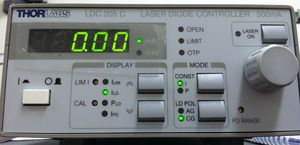
\includegraphics[width=0.5\linewidth]{images/300px-QIE_LDController.jpg}}
    \caption{Thorlabs LDC 205 C Diode Laser Controller.}
    \label{fig:300px-QIE_LDController}
\end{figure}

\textbf{Note: Do NOT put the power meter next to the Laser Diode, Only measure power after the optical Isolator.}

The experiment is powered by a \href{http://experimentationlab.berkeley.edu/sites/default/files/QIE/D405-120.pdf}{\textbf{120-mW, 405-nm violet diode laser}}, the same wavelength used by Blu-ray Disc\textsuperscript{TM} players. \textbf{This is a Class 3B laser and can cause permanent eye damage if the beam directly enters the eye. DO NOT REMOVE THE 405 BANDSTOP FILTER AT THE END OF THE DOWN-CONVERSION SOURCE (BBO CRYSTALS) OR THE ORANGE BEAM ENCLOSURES THAT PREVENT STRAY REFLECTIONS FROM LEAVING THE BEAM PATH.} Orange protective goggles are available by the door.

Because this is a diode laser, all the photons in the beam have the same polarization, in this case horizontal. The laser beam incident on the BBOs (i.e., after the intermediate optics) is sometimes referred to as the ``pump'' beam.

\textbf{Before you turn on the laser, make sure that the Temperature Controller next to the Laser Diode Controller is on. If not, turn it on.}

The diode laser is powered by a Thorlabs LDC205C diode laser controller, located on top of the optical bench roof. Turn the controller on with the switch in the lower left corner. We run the laser diode in constant current mode and cathode ground (CG) polarity. You will want to view the laser diode current, ILD. To operate the diode, use the button in the upper right corner to turn it on and turn the knob to control the current. Any time the laser diode is on, the light on the QIE room door will be flashing red. The current limit is set to 100 mA to avoid burning out the diode. If you reach this limit, the controller will beep, the red ``LIMIT'' LED will turn on, and you will not be able to increase the current further. However, it is okay to run the laser diode at its maximum current.

Right after the laser diode, there is an optical isolator which prevents light reflected further down stream from going back into the diode. Isolators are used to reduce or eliminate the effects of optical feedback: reflections of a laser’s energy back into itself. These effects include noise, amplitude fluctuation, and laser damage. Isolators protect the laser, while maintaining beam alignment and providing maximum forward transmission and reverse isolation. Laser light enters the isolator via the input polarizer and is linearly polarized. This light then enters the rotator, which rotates the plane of polarization +45$^\circ$. The beam exits through the output polarizer, whose axis is oriented +45$^\circ$.

The isolator used is supposed to have a transmission efficiency of 84\%. It is worth while to check for yourself (using a power meter before and after the isolator) to see if the efficiency is at least close to the expected. If it is not, you may need to realign the polarization optics. \textbf{It is unlikely you need to do this}, but if you do, 1) Loosen the cap screw holding the isolator in the slip ring. (in the side facing away from the laser diode). 2) Rotate the isolator until transmission is maximized. This occurs when the input polarizer is aligned to the laser’s plane of polarization. Lock down the slip ring cap screw.

To monitor the behavior of the laser diode, every student is asked to measure the 405 nm laser light power as a function of the supplied current. Use a power meter, measure power after the optical Isolator, (ask the staff if you cannot find it in the room. The meter is shared among many experiments.) Start from 0 mA (or the lowest you can get) and measure the power of 405 nm laser light right after the optical isolator. Make sure the wavelength setting of the power meter is set to 405 nm (why?). Measure up to 100 mA. Include the plot in your lab report.

\subsection{BBOs}

\begin{figure}[h]
    \centering
    \href{http://experimentationlab.berkeley.edu/sites/default/files/violetbeamdiagram2.jpg}{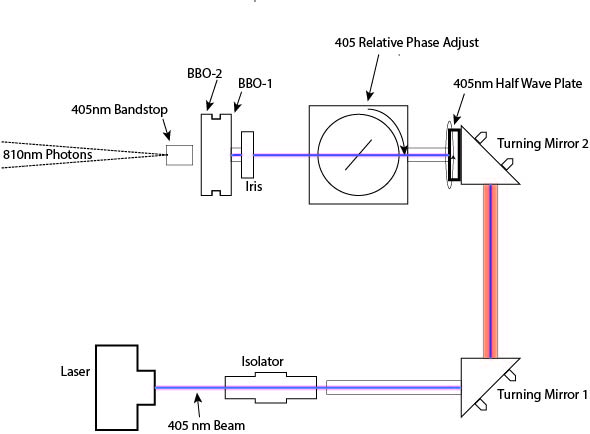
\includegraphics[width=0.5\linewidth]{images/violetbeamdiagram2.jpg}}
    \caption{Diagram of violet beam path optics. Updated 2016.}
\end{figure}

\textbf{IMPORTANT: As of 2016, it is not possible to rotate the BBO optical axes relative to each other.}

The beam passes through some optics (two steering mirrors, two wave plates, and an iris -- see \href[sec:Alignment]{Alignment}) before reaching the pair of nonlinear beta barium borate ($\beta$-BaB2O4 or just BBO) crystals. When a pump photon of a particular polarization enters such a BBO crystal, it can be converted into two photons each with (about) half the initial energy of the pump photon (and twice the wavelength = 810 nm). These photons exit the crystal symmetrically at a small angle. Often those photons referred to as the ``signal'' and ``idler'' photons, but we can just as well call them the A and B photons, referring to the two arms of the detection setup along which they will travel. Most importantly, their polarization is entangled, meaning that the photons are guaranteed to have (in this case) the same polarization.

Note that the two beams of the down-converted photons will not be visible to the naked eye because (1) the wavelength of 810-nm photons are infrared and (2) the beams are extremely low-power as the conversion efficiency of the crystals is quite small. (Think about how much power $\sim$1,000 photons per second correspond to and compare this to the laser diode power rating.)

\begin{figure}[h]
    \centering
    \href{http://experimentationlab.berkeley.edu/sites/default/files/qie_optics_image_0.jpg}{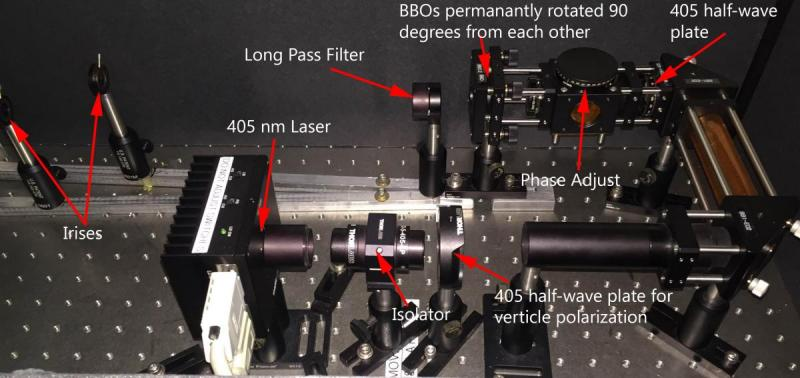
\includegraphics[width=0.7\linewidth]{images/qie_optics_image_0.jpg}}
    \caption{Photo of violet beam path optics.}
    \label{fig:qie_optics_image_0}
\end{figure}

Two BBO crystals are mounted with their optical axis aligned perpendicular to each other. Each BBO crystal converts only photons of a single polarization. Because the separation between the BBOs is so small, the down-converted photons from each BBO essentially travel along the same cone to the detectors. This means that the horizontally polarized pairs are indistinguishable from the vertically polarized pairs until we perform a polarization measurement on them. In a quantum mechanical picture, each pair of down-converted photons is in a superposition of vertical and horizontal polarization until a measurement collapses the wavefunction into one state or the other. The evolution of the quantum state of the system from emission to down-conversion is summarized below in bracket notation \textbf{with the assumption that the BBOs are perpendicular}. $H$ and $V$ refer to horizontally and vertically polarized states of a pump photon, respectively, and $h$ and $v$ refer to horizontally and vertically polarized states of a down-converted photon. $hh$ and $vv$ are short for the combined state of a pair of down-converted photons, and $\psi$ is the polarization angle of the pump beam. Thus, each BBO can act on the pump photon in the following manner:
\begin{gather*}
    \text{BBO-1: } |V\rangle \rightarrow  |vv\rangle \\
    \text{BBO-2: } |H\rangle \rightarrow  |hh\rangle 
\end{gather*}
Assuming blue pump light with its polarization described by $\sin \varphi |V\rangle + \cos\varphi e^{-i\delta} |H\rangle$, we arrive at $|\Psi\rangle = \sin\varphi |vv\rangle + \cos\varphi e^{-i\delta} |hh\rangle$.

The probability of detecting a given polarization depends on the polarization of the pump laser. You can adjust the polarization of the pump laser by rotating the 405-nm half-wave plate located between the two steering mirrors.

We have installed a 405-nm band-stop filter after the BBOs for laser safety reasons. Although approximately 50 mW of power are incident on the BBOs, the filter attenuates this to less than 1 mW. This power can be viewed safely in order to align the detection components. Therefore you do not need to wear laser safety goggles if this band-stop filter is installed AND no pump light is leaking out of encased area before the band-stop.

\subsection{Detection}

\begin{figure}[h]
    \centering
    \href{http://experimentationlab.berkeley.edu/sites/default/files/images/IMG_4032.jpg}{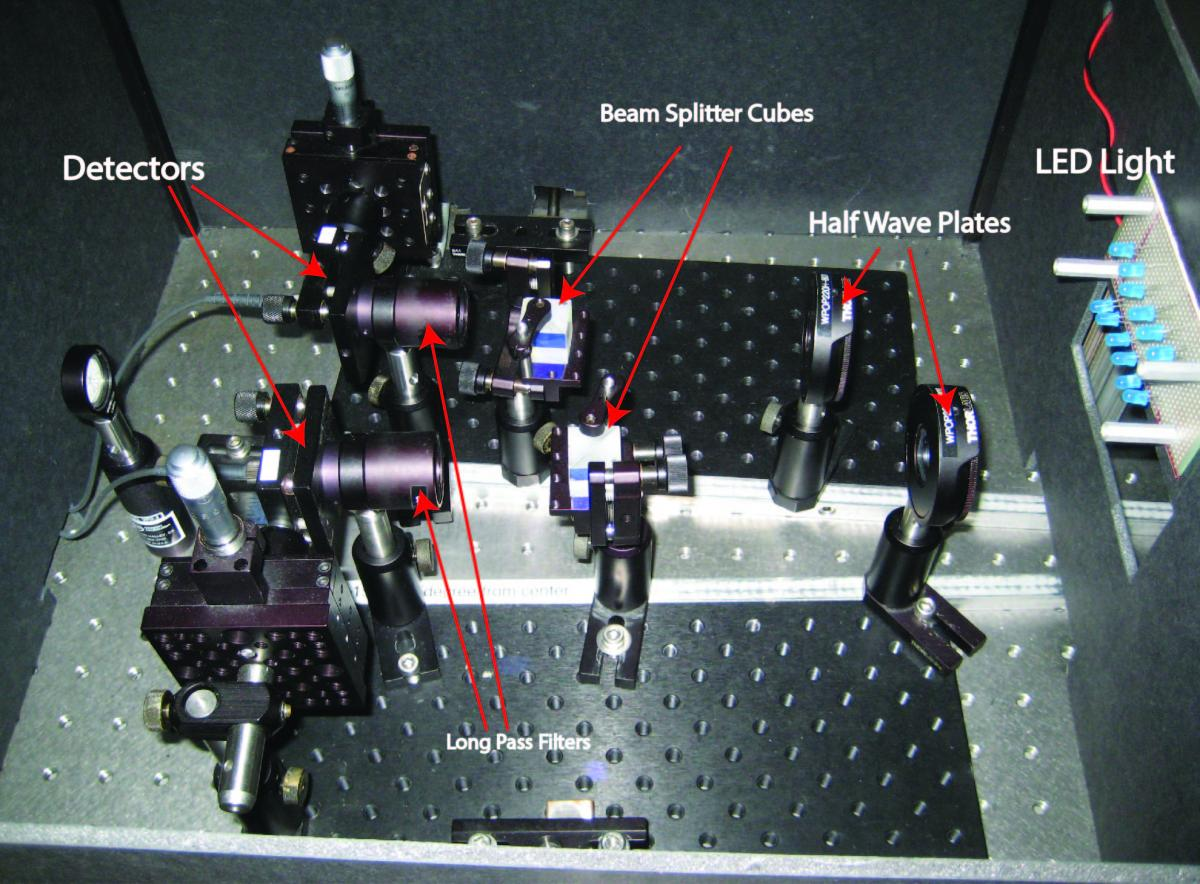
\includegraphics[width=0.5\linewidth]{images/IMG_4032.jpg}}
    \caption{Detection arms from the front of the box.}
    \label{fig:IMG_4032}
\end{figure}

The detection setup consists of two identical arms separated by a small angle. The angle can be adjusted to match the trajectory of the down-converted photons and should be centered around the violet laser beam.

Each of our detectors consists of a small fiber coupler (FC) lens, which focuses the light into an optical fiber. The optical fiber runs from the lens to an avalanche photodiode (APD), which converts single photons into sizable ($\sim$1 V) electronic pulses. They can detect anywhere from hundreds of photons to tens of millions of photons per second. The APDs are powered by a homemade power supply, located above the APDs on the optical bench roof. The power supply has a master on/off switch and four switches to turn the APDs on and off individually. \textbf{An alarm within the APD power supply will alert you if you are overloading the APDs. If you ever hear this, immediately turn off the APDs to prevent damage.} Ambient light conditions are typically okay as long as you \textbf{do not remove the long-pass filter on the detectors while the APDs are on.}Note, however, that this alarm sounds for several seconds every time the APDs are turned on. This is normal.

To measure the polarization of the photon pairs, each detection arm has a half-wave plate to set the measurement basis and a polarizing beam splitter cube. The beam splitter allows horizontally polarized light to pass and reflects vertically polarized light out at 90$^\circ$. This setup only allows photons to reach a given detector if they have a certain polarization (or, equivalently, their arrival at a given detector means that their wavefunctions have collapsed into a given polarization state). In other words, the beam splitter makes the horizontally polarized photons distinguishable from the vertically polarized photons. Please note that there most probably is an arbitrary offset between the reading on the mounts for the half-wave plates and the actual direction of the optical axis of the half-wave plate. Think about a way you can find the ``zero'' of the two half-wave plates by pumping only one crystal at a time (i.e. by sending in only vertically or only horizontally polarized light into the BBOs rather than a superposition of both), removing both of the half-wave plates and then placing one at a time while varying the angle. You should be tracking the coincidence counts throughout this process. Remember that the beam splitters only let through one polarization of light. You can use this fact to zero the half-wave plates. \textbf{This procedure will have to be done after you are receiving coincidence counts. }

\subsection{Coincidence Counting}

Signals from the APDs are sent to a field-programmable gate array (FPGA) [\href{http://www.altera.com/education/univ/unv-index.html}{\textbf{Altera DE-2}}] that has been programmed to calculate coincidences. A coincidence is the arrival of two photons at different detectors within a short coincidence window, typically 5 ns for our setup. The FPGA sends photon counts for each detector and coincidence counts for each pair of detectors to LabVIEW, which displays the data on the thermometer-like indicators on the front panel. These data can be used to calculate $S$.

\subsection{Proper Start-up Procedure}

\noindent
\href{http://experimentationlab.berkeley.edu/sites/default/files/images/QIE1.jpg}{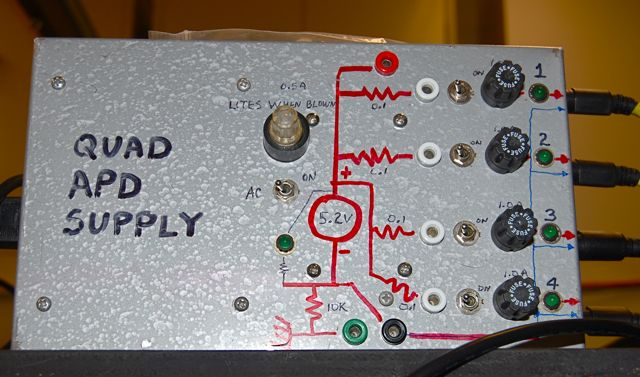
\includegraphics[width=0.25\linewidth,keepaspectratio]{images/QIE1.jpg}}
\href{http://experimentationlab.berkeley.edu/sites/default/files/images/QIE4.jpg}{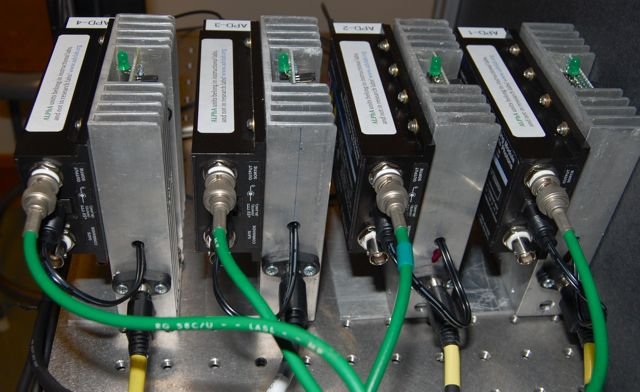
\includegraphics[width=0.25\linewidth,keepaspectratio]{images/QIE4.jpg}}
\href{http://experimentationlab.berkeley.edu/sites/default/files/images/QIE3.jpg}{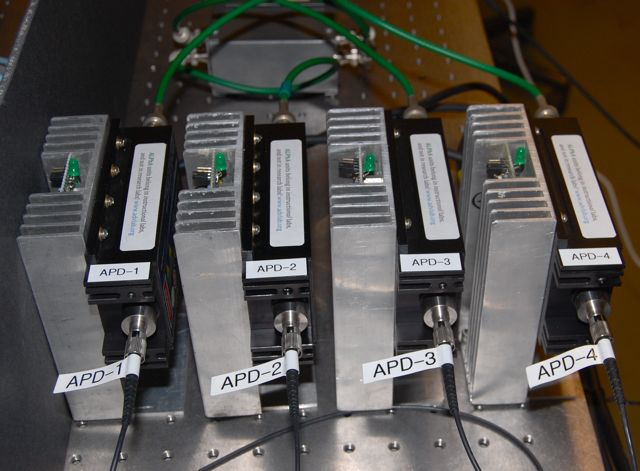
\includegraphics[width=0.25\linewidth,keepaspectratio]{images/QIE3.jpg}}
\href{http://experimentationlab.berkeley.edu/sites/default/files/images/QIE2.jpg}{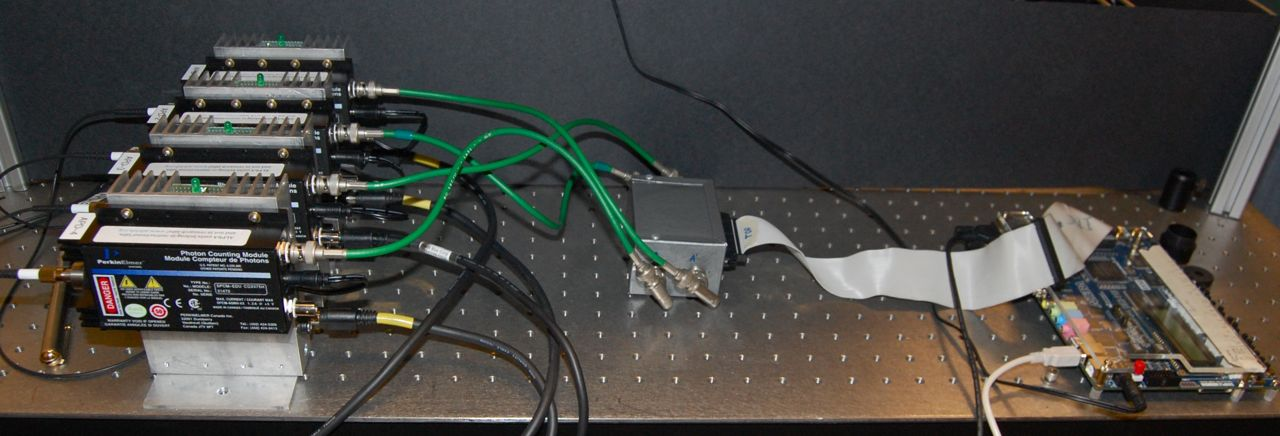
\includegraphics[width=0.25\linewidth,keepaspectratio]{images/QIE2.jpg}}

\noindent Due to the idiosyncrasies of our software, it is important to follow these steps in the correct order:

\begin{enumerate}
    \item Turn on the computer and log in.

    \item Turn on the FPGA.

    \item Run the LabVIEW program (latest version: C:\textbackslash QIE\_Counter\textbackslash QIE Counter.exe, see \href[subsec:UsingLabVIEWProgram]{using LabVIEW}).
\end{enumerate}

If you turn the FPGA on before the computer, you may not be able to use the mouse. If you run LabVIEW before turning on the FPGA, you will get an error message.

The APDs can be turned on and off at any time, but you should be aware that turning them on while the lights are on influences your results (check this out). Therefore we encourage you not to turn the APDs on while the lights are turned on. It is usually best practice to turn on the main switch to the APD power supply (on the left) and then turn each APD on individually. This allows you to know which APD is overloaded should the alarm sound continuously. Remember that it is normal for the alarm to sound for a few seconds as each APD is switched on.

\section{Alignment}
\label{sec:Alignment}

Because our detector apertures are only a few mm in diameter, proper alignment is essential to obtaining good data.

\subsection{Violet Beam Path}

We are using an optical cage system between the laser diode and the BBOs to make alignment of this portion of the beam path fairly simple, as well as to ensure laser safety. The orange material around most of the beam path attenuates the laser power enough to be safely viewed by the naked eye but not so much as to obscure the view of the laser dot from the outside. If this material ever glows enough to add significant noise to your data, block the detectors' view of it with the black shields.

The following alignment procedure is based on height of the paper target behind the detector arms being correct. In theory, this target never needs to be moved or adjusted. However, if you notice that the target height seems drastically different than the height of the violet beam, you will need to adjust the violet beam path direction.

We want the beam of the violet laser to go through the center of both of the BBO crystals as well go through the center as defined by both detectors, i.e. the target near the detectors. For this portion of the calibration you should be using your protective goggles. First, with the laser on, turn down the power to the violet laser using the knob on the laser diode controller. On the rear face of the BBOs (the face closer to the detectors) there should be a bandstop filter designed to filter out the violate light. Remove the filter. Do not turn the laser up too high now that the filter is removed as it could damage your vision. Next place one of the circular paper targets where the filter was. The center of the paper target will be one of the points we will be calibrating the first stage of the optics to.

Carefully turn up the power on the laser until it is faintly visible (without your glasses) on the paper target attached to the BBOs. If you don't see the dot from the laser at any power setting, open the iris just in front of the BBOs. If that does not help, the front two mirrors are completely misaligned. At this point it will be much easier to work without your glasses, but make sure the laser power is low enough that you won't damage your eyes and that you avoid looking down the beam path regardless.

Use the two turning mirrors to aim the beam down the center of the optical cage to the paper target behind the detectors. Because the first mirror is farther upstream, it is a finer adjustment to the beam spot's position on the BBOs. Use the first mirror to guide the beam to center the beam on the target (and the iris), use the second mirror to guide the laser beam to the center target near the detectors. Repeat the process until you have the beam accurately centered on both the BBOs and the target. Once the laser is aligned, you can open the iris in front of the BBOs all the way or leave it partially closed as you see fit.

Important: at this point it is also wise to check the tilt of the half waveplate (used for the phase adjustment) between the halfwave plate (used for pump beam polarization) and the second mirror. Make sure that it is roughly perpendicular to the beam path to begin with and then optimize its angle with respect to the incident blue laser beam. Angles greater than 45 degrees will limit your observable coincidence rates severely.

\textbf{Potentially useful additional alignment details -} Check to make sure that the laser spot coming out of the BBOs is a focused to a spot. It should not look like a line. If it does look like a line, the focus of the laser needs adjusting. Only do this with an instructor. Together with the instructor, adjust the focus by \textbf{CAREFULLY} removing the protective cover of the laser diode by unscrewing it from the front (it looks like a small black tube protruding from the black box that holds the laser diode). This will expose the lens, which can be focused by turning it. You should change the focus slowly while viewing the laser exiting the BBOs. Focus the laser to a spot as best as possible.


\textbf{This is a Checkpoint:} \emph{Show a GSI or Professor that you have properly calibrated the Violet Beam Path. This can be demonstrated by focusing the beam on the target located at the back of the detector, between the two detection arms. Also demonstrate that you know how to hook and unhook the Fiber Optic cables to the Infrared laser as well as the FPGAs. Some more information and pictures of the Fiber Optic cables are located in the Infrared Beam Path section below.}

\subsection{Infrared Beam Path}

This is a \href{http://experimentationlab.berkeley.edu/sites/default/files/QIE/laser.JPG}{\textbf{picture}} of the infrared laser you should be using. It is a portable, black, cylindrical tube that can fit in your hand.

Align the components on each detector arm independently of the other arm using the following procedure. During this procedure, you will have to remove the optical fibers from the APDs. Make sure the APDs are turned off before you do this. Allowing ambient light to enter the APDs directly will overload them. \textbf{Be careful not to clamp anything down on top of the optical fibers during alignment. They are fragile and expensive to replace. When plugging into the FPGA a little tooth must be aligned with the port in order to be properly connected. you should not have to force the connection. There are pictures located below }\textbf{of the tooth and }\textbf{of the port for the FPGA. However, when plugging the fiber optic cable no tooth alignment is necessary, so we have also included a }\textbf{of the port of the laser where the optical cable is inserted. Along similar lines: don't pull on the jacket (the black cover), instead carefully wiggle on the metal connector itself to remove the fiber from the connection. In addition, make sure that you do not scratch the front facets. The fibers are really fragile and they are also expensive, so simply do not break them!}

\noindent
\href{http://experimentationlab.berkeley.edu/sites/default/files/QIE/fiberopticcable_0_0_1.JPG}{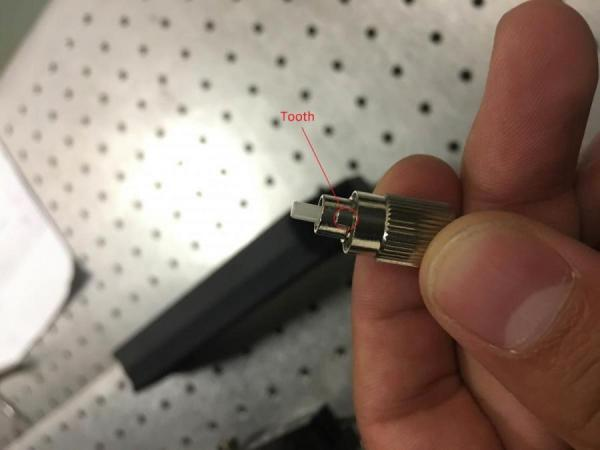
\includegraphics[width=0.33\linewidth,keepaspectratio]{images/fiberopticcable_0_0_1.JPG}}
\href{http://experimentationlab.berkeley.edu/sites/default/files/QIE/fpgaport_0_1.JPG}{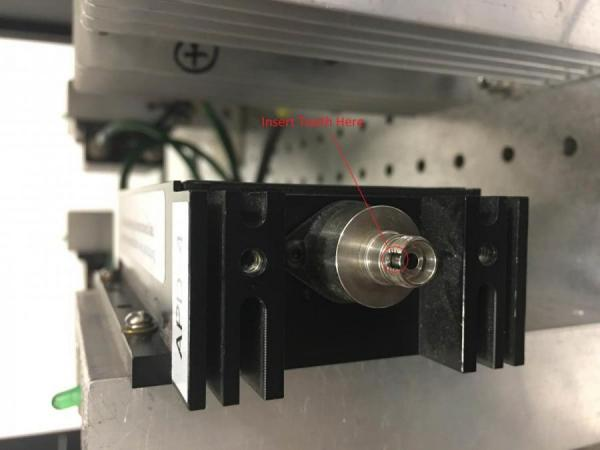
\includegraphics[width=0.33\linewidth,keepaspectratio]{images/fpgaport_0_1.JPG}}
\href{http://experimentationlab.berkeley.edu/sites/default/files/QIE/insertend_0_1.JPG}{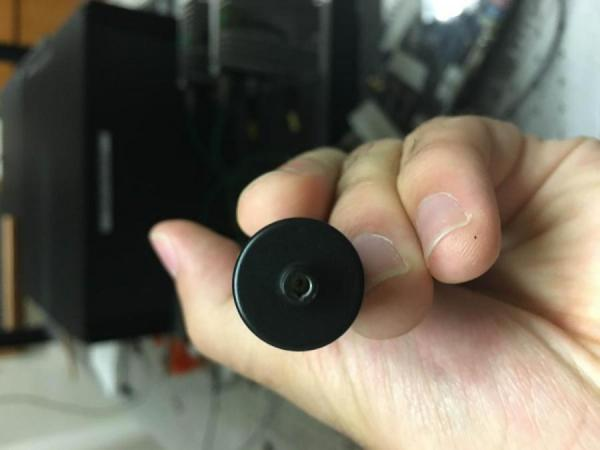
\includegraphics[width=0.33\linewidth,keepaspectratio]{images/insertend_0_1.JPG}}

Goal will be to align the detectors such that they ``look'' at the BBOs where the entangled photon pairs are created. For this, we will send a test beam in the opposite direction through the fibers and the collimation optics and try to match the path of this test beam and the path the downconverted photons will take to each other. Note that the light needs to be focused into the core of a multi-mode fiber whose diameter is on the order of 100 $\mu$m. That means that precise alignment is critical.

\begin{enumerate}
    \item First we remove the beam splitter cubes, half-wave plates, and the long-pass filters from the detectors.

    \item Remove the optical fiber from the APD and connect it to the red fiber testing laser (looks like a laser pointer). The resulting red light cone represents all the light that will be collected by the detector in your experiment. The size of the red-light cone should not be much larger than the diameter of the BBOs. If the laser light is not collimated properly, there must be a problem with the port. There is a circular rubber holder that may be misaligned. It is important that you do not try to fix this problem yourself and you should call over the professor to fix the problem.

    \item By making small adjustments using either the screws on the back of the detector or your hand, your goal is to aim the test laser as precisely  as possible at the center of the BBOs. With the red laser and the blue laser on, the two spots should overlap at the BBOs.
    
    \textbf{Detector A/B Height:} Swing the detector arm to the center so that the violet beam is centered horizontally on the target. First move the plate on which the detectors are mounted parallel to the back plate with the thumb screws on the back of the detectors. Later, this will allow you to adjust the angle of the detectors in all directions with the thumb screws. Then adjust the height of the detector so that the violet beam passes through the pinhole, i.e., the red and violet beams coincide. Later on, you might be able compensate for slight vertical misalignment by adjusting the second turning mirror in the violet laser path to optimize count rates. However, it may be difficult to optimize this way for both detectors.
    
    \textbf{Detector A/B Angle:} Adjust the thumb screws on the back of the detector until the red circle is well centered on the BBOs. You can use a piece of white paper to see the beam if it helps. If necessary, you can also adjust the thumb screws on the BBOs so that the back-reflection of the red circle is centered on the detector aperture. These thumb screws move both BBOs together. However, it may be difficult to align this back reflection for both arms. Note that the position of the red-cone will change when you rotate the arms (why is that?). So should think about how to set the detector arm angles and then readjust as necessary.

    \item Replace the long-pass filters on each detector and reconnect the optical fibers to their corresponding APDs. Make sure when reconnecting the fibers that the notch on the connector is lined up correctly. You will not be able to insert the fiber all the way in if it is not aligned, meaning light could possibly leak in and out.

\end{enumerate}

\subsection{Detection Arm Angle}

The optimal angle for the detection arms will be the angle at which AB coincidences are maximized. Use the micrometers to vary the angle of each arm until you find a setting that \textbf{maximizes coincidences}. Make a note of the exact readings, although you should not need to move these arms again.

\textbf{This is a Checkpoint}: \emph{Show a GSI or Professor the angle that you expect a maximum of the red-photon counts on single arm. Is there a chance to observe coincidences for any pair of angles?}

Having successfully answered the above question you should quickly find substantial coincidence rates well above 800 counts/s. Now you may want to try to enhance the coincidence rate by adjusting all parameters.

\subsection{Inserting the polarization analyzing elements}

The photons will be entangled in the polarization degree-of-freedom. Therefore, will will have to analyze the polarization with a combination of a polarizer (polarizing beam splitter cube) and a half-wave plate. For this you can either use the red alignment laser or swing the arms into the center such that you can use the blue beam as guidance. If you have a good eye you can also get away with just inserting them into the path, but be aware that if you make a mistake you will severely limit the number of coincidence as well as the quality of the polarization analysis.

\begin{enumerate}
    \item \textbf{Cube Position:} Insert the beam splitter with the front face (marked by a dot on top of the cube) towards the BBOs. (There is only one correct position for the dot.) Adjust its position and height so that the red beam passes roughly through the center of the back face.

    \item \textbf{Cube Angle:} Adjust the thumb screws on the cube mount so that the light gets reflected straight back into itself. For this you might want to punch a whole into a sheet of paper and hold it into the beam path.

    \item \textbf{Half-Wave Plate A/B:} Insert the half-wave plate in front of the beam splitter. Adjust the position and angle with respect to the laser beam axis the same way as with the beam splitter.
\end{enumerate}

For most settings of the halfwave plates, you should see already coincidences. However, you might want to reoptimize the angle settings of the detector arms. Why?

\textbf{This is a checkpoint:} \emph{By now you should have your experimental setup fairly aligned and reading coincidences. Show a GSI or Professor that you have properly aligned the setup. Demonstrate that the infrared beam path and the violet beam path emerging from the BBO crystals converge (i.e. that the system is aligned). You should be done with the alignment by the second day. If you are not, it means you are falling behind and may want to call over a GSI or Professor for some help.}

\section{Producing a Bell State}

A Bell state is a maximally entangled state of two qubits, namely
\begin{equation}
    |\psi^\pm\rangle = \frac{1}{\sqrt{2}}(|hh\rangle \pm |vv\rangle)
    \quad \text{or} \quad
    |\phi^\pm\rangle = \frac{1}{\sqrt{2}}(|hv\rangle \pm |vh\rangle).
\end{equation}
(Note that we can only produce the $\psi$ states because our BBOs down-convert into pairs with like polarization.) Ideally, we would like each pair of down-converted photons in this experiment to be in a Bell state. However, many factors can contribute to deviations from perfect entanglement:

\begin{enumerate}
    \item pump beam not polarized at 45$^\circ$

    \item phase shift due to BBOs

    \item separation between BBOs

    \item angle between BBOs

    \item different down-conversion efficiencies of BBOs
\end{enumerate}
In particular item 2 needs some explanation. A small phase shift between the horizontally and vertically polarized photon pairs can occur due to dispersion and birefringence in the BBOs. (You can also think of this as adding a slight elliptical polarization to linearly polarized light.) Let's say that instead of producing a perfect Bell state, the BBOs introduce a small relative phase shift $\delta$:
\begin{equation}
    |\psi\rangle = \frac{1}{\sqrt{2}} (|hh\rangle + e^{i\delta} |vv\rangle).
\end{equation}
This would decrease the number of coincidences when the state is analyzed in a diagonal basis (see prelab). To compensate for this, we need to delay one component of the pump beam by $\delta$ before it reaches the BBOs. We can do this with a birefringent crystal. We have chosen to use a half-wave plate rotated about the vertical (so that it functions as a less-than-half-wave plate). The half-wave plate is installed on a rotational mount with its optical axis parallel to the vertical. When the rotational mount reads 0$^\circ$, the laser beam is perpendicular to the face of the wave plate. Rotate this wave plate such that you produce an ideal Bell state with $\delta$ = 0. For this you can choose particular settings of the halfwaveplates in the analyzing paths or you can record the coincidences for a range of the two analyzer half waveplate settings (see midlab question). However, note that the analysing halfwave plates might not be calibrated properly, i.e. a reading of 0 degrees might not correspond to the optical axis of the waveplate to be aligned in the same direction. If you suspect this, calibrate the offset in both waveplates by using a test laser and two orthogonally oriented polarizers.

The separation between the BBOs is small enough to be negligible, and as noted above, the angle between the BBOs is practically eliminated when the BBOs are at 90$^\circ$. We cannot control the down-conversion efficiencies of the BBOs, but they should be very similar.

\textbf{This is a checkpoint:} \emph{Using the knowledge that the polarizing beam splitters (PBS) only allow one linear polarization of light into the detectors and the fact that the BBO optical axes are rotated 90 degrees from each other, think of a way to ensure that you are pumping only one of the two crystals (one BBO). From here you should be able to calibrate the 405 nm half-wave plate controlling. You should do this and record the calibration. Call over a GSI or Professor and show them a final value for the arbitrary offset of each Half Wave Plate. Explain how you were able to find this offset. (This process was described at the end of the ``detection'' section located above).}

\subsection{Mid-Lab Questions}

Before going on, we are interested in verifying that everything in the experimental setup is doing what we think it is doing, or is supposed to be doing. We will start with the half-wave plates, which should have been calibrated in a previous checkpoint. The ones of concern are the 405nm half-wave plate controlling $\theta_l$ and the half-wave plates angles for the detector arms.

The first thing to test towards figuring out the purity of your bell state should be the dependence of the coincidence rates on the settings of the two half-wave plates attached to your detector arms. To fully explore what's going on, you will need to make several plots. Watching only the readings for the individual detectors A and B, you will vary the angles of the half wave plates along the detection arms.

\textbf{Before doing this} note in your notebook what you expect. If the system is working correctly, how do you expect the individual readings to change as you vary the measurement basis(i.e. the two angles of the half wave plates along the arms)? Think about what the half wave plate and beam splitter are really doing and write down your prediction (this goes back to the technique used to measure the offset of the HWP). Test your prediction. Explain. Include this analysis in your write-up.

Calculate the contrast (max(coincidences)-min(coincidences))/(max(coincidences)+min(coincidences)) for the half wave plate along detector arm A at two fixed angles, 0 and 45 degrees (due to the nature of the halfwave plate this will induce a 90 degree phase shift in the incoming wave, if you do not understand this then refer to the optics tutorial linked at the start of the lab), and varying the angle of the other half wave plate located along detector arm B. What can you say from this about the purity and/or fidelity of your Bell state? Do you expect these contrasts to be equal? If they are not, what is your explanation? The contrasts in your data have to do with the vh and hv states.

Once you understand what is going on you should plot the coincidence rates  as a function of the angle of one of the two half-wave plates (keeping the other one fixed). Repeat this measurement for roughly 4 different fixed angles (You can find out which four angles would give you the best intuition of your bell state by reading Dehlinger and Mitchell \cite{Dehlinger}).

A few tips for understanding your bell state and understanding which characteristics are important:

\begin{itemize}
    \item The span for each of the four data sets, not only the 0 and 45 degree angles, should be roughly the same (you can varying this using the Half-Wave and Quarter-Wave plate settings of the violet beam path). Keep in mind that the other fixed angles will inform you of the entanglement of your state;

    \item The phase shifts in the fitted data should correspond to the phase shifts induced by the rotation of the half-wave plate that is fixed to an angle;
\end{itemize}

Make sure you understand what you expect to see for each plot, and ask an instructor if you are unsure. If you find that you do not have a reasonable Bell state, use the plots you created to figure out which parameters need adjustment. Adjust these and retake the data until you create the state you are aiming at. Alignment adjustments can also help improve counts on detectors that seem to be missing photons, however if you receiving good counts before this is unlikely to be the culprit.

Dehlinger and Mitchell \cite{Dehlinger} is a good resource for tuning your Bell state.

Once you have recorded four good sets of data, plot them against each other and see what you can gather from these measurements about the phase $\delta$ of the Bell state $|\psi \rangle = \frac{1}{\sqrt{2}} (|hh\rangle + e^{i\delta} |vv\rangle)$? If unsure, use the little program you wrote for the prelab and plot the expected coincidence rate as a function of various angles of the half wave plate detectors along the detection arms. Do the points of your data align with the fit? Note that it will be absolutely crucial that you understand what is going on at this stage before you proceed.

\subsection{Quantifying your Bell State}

This section of the lab is very beneficial to your understanding of the experiment, however, not crucial for completing the experiment. You must attempt to violate Bell's Inequality (next section) in order to complete the lab, so if you short it time you might consider skipping this.

We are interested in determining and quantifying the photon state we have created as it is likely not a perfect Bell state. Assuming it is of the form $|\psi_{DC}\rangle = C_1 |hh\rangle + C_2 e^{i\phi}|vv\rangle$. It is your task to determine $C_1, C_2$ and $\phi$.

\textbf{This is a Checkpoint}: \emph{Assume indistinguishable particles. Show a GSI or Professor that the measurements you have to make to measure $C_1, C_2$. Which for determining $\phi$? Refer to Dehlinger and Mitchell \cite{Dehlinger} if unsure.}

Until this point, we have assumed indistinguishable particles. What element of the experimental setup determines if this is truly the case? In other words, how are the photons created to be indistinguishable in a super position of $|vv\rangle$and $|hh\rangle$. If they are not truly indistinguishable, then you can assume that the photon pairs are either $|vv\rangle$ or $|hh\rangle$. What consequences does this have for your coincidence measurements as a function of the angles $\alpha, \beta$? Based on your analysis: how can we test for distinguishability in our setup?

\section{Violating Bell's Inequality}

Four angle pairs are needed for each $E$ measurement. (The E Meter in LabVIEW program is meaningless at this time.) You essentially need to adjust the half-wave plates to redirect photons to the A and B detectors that would otherwise have been reflected by the beam splitters. If you need help figuring out which angle pairs to use, see the paper by Dehlinger and Mitchell \cite{Dehlinger}.

\subsection{Using the LabVIEW Program}
\label{subsec:UsingLabVIEWProgram}

The most recent version of the LabVIEW program is C:\textbackslash QIE\_Counter\textbackslash QIE Counter.exe. Make sure the FPGA is powered on before you run LabVIEW or you will get an error message. Upon running the vi, you should see the front panel below.

\begin{figure}[h]
    \centering
    \href{http://experimentationlab.berkeley.edu/sites/default/files/images/600px-QIE_LabVIEW.png}{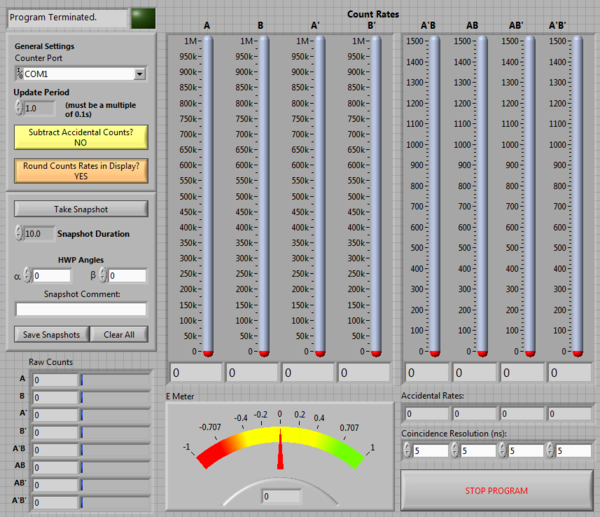
\includegraphics[width=0.5\linewidth]{images/600px-QIE_LabVIEW.png}}
    \caption{Front panel of QIE\_Counter.vi}
    \label{fig:600px-QIE_LabVIEW}
\end{figure}

\subsubsection{Count Rate Indicators}

If you have the APDs powered on, the first thing you will notice is the eight large ``thermometer'' indicators. These display count rates on each of the four detectors (at left) and coincidence rates for each pair of detectors (at right). The count rates are calculated by dividing the raw counts from each of the FPGA registers, shown in a column vector at the bottom of the screen, by the update period, controlled in the General Settings box. \textbf{[Since only two detectors are being used in the experiment at this time, some of the indicators are irrelevant in your measurement.]}

Below the coincidence rates are the accidental rates, calculated using the coincidence resolution controls on the following line. You should have derived the formula for this calculation in the pre-lab. The values in the coincidence resolution array may or may not agree with the actual coincidence window used by the FPGA. This is controlled by a physical switch on the FPGA, but it also tends to drift from its nominal value. Keep in mind that the accidental rates are only as accurate as the coincidence resolutions.

To the left of the coincidence resolutions is the E Meter. $E$ is calculated as described in the \href[sec:Introduction]{Introduction}. Note that $E$ can only be calculated if all four detectors are being used simultaneously.

To the left of the E Meter are the Raw Counts indicators. You can verify that the count rates are indeed the raw counts divided by the update period.

\subsubsection{Status Indicators}

In the upper left corner, you will see the status indicators. The text box has five possible values:

\textbf{Initializing}

LabVIEW is starting up and connecting to the FPGA.

\textbf{Reading Counters...}

LabVIEW is waiting for one Update Period to elapse.

\textbf{Updated Counts}

LabVIEW has read the FPGA registers and recalculated count rates. The green rectangle flashes once each time this occurs.

\textbf{Closing Program...}

You have clicked the Stop Program button.

\textbf{Program Terminated.}

The vi is not running.

\subsubsection{General Settings}

``Counter Port'' should be set to COM1 in order to connect to the FPGA.

``Update Period'' controls how long LabVIEW will wait between buffer reads. In other words, it will count photons for this amount of time and then display the resulting count rates.

The ``Subtract Accidental Counts?'' button toggles whether or not LabVIEW will subtract the values in the ``Accidental Rates'' array from their respective coincidence rates. Note that there is a lag time of one cycle between when you click this button and when LabVIEW actually starts subtracting.

The ``Round Count Rates in Display?'' button toggles rounding in the eight thermometer indicators. This can be useful because dividing by the update period often gives fractional count rates. Note that this function also exhibits a lag time of one cycle.

\subsubsection{Snapshots}

Snapshots allow you to take data points and save them to a file. ``Snapshot Duration'' is the length of time, in seconds, of the snapshot. You also have the option to enter angles for half-wave plates A and B and a comment, which will be saved with the snapshot. When you click ``Take Snapshot'' for the first time, a new window will pop up displaying the data you have taken. Each subsequent time you click ``Take Snapshot,'' a row will be added to the new window. When you are done taking snapshots, click ``Save Snapshots'' in the main window. To clear the pop-up window for a new set of snapshots, click ``Clear All.''

To avoid any false coincidences we suggest that you turn off the lights and monitor before taking snapshots. If your duration is longer than three seconds, it's easier to use some kind of timer, for instance \href{http://www.timeanddate.com/timer/#}{\textbf{http://www.timeanddate.com/timer/\#}} .


\section{After the Experiment}

Make sure all of the following equipment is powered down at the end of each day:

\begin{itemize}
    \item laser controller

    \item APD power supply (turn all five switches off)

    \item FPGA

    \item computer, monitor, speakers

    \item room lights

    \item Last day of the experiment please fill out the \href{\ExperimentEvaluation}{\textbf{Experiment Evaluation}}

\end{itemize}

\section{Extensions}

\subsection{Double slit quantum eraser}

Before conducting the quantum eraser experiment as described by Walborn et al \cite{Walborn}, you should perform a single photon double slit experiment. For this you only need to consider detector A. Please follow the steps to align the beam path.

\begin{enumerate}
    \item Center \textbf{detector A} by turning the micrometer to 0 mm and using the inch micrometer (from now on called inchmeter) and screw-on target. Take notice of the position of the inchmeter.

    \item Mount an \textbf{iris} onto the black optical board and align it so the violet beams passes the iris when closed.

    \item Remove the screw-on target and carefully screw the \textbf{200 $\mu$m slit} on top of the 800 nm bandwidth filter. (There is one particular filter which has been set further into the black tube.) Screw the filter with the slit back on detector A as far as possible with the slit being vertically aligned.

    \item Use the micrometer to find the \textbf{ideal position of the detector}. Take a few measurements (10s each) and then fit a Gaussian.

    \item Put the micrometer to the position of the calculated peak and \textbf{adjust the angle} until you reach the highest possible count rate. The iris in front of the BBOs should be closed and the one downstream opened.

    \item Center your detector again (micrometer should read 0 mm) and put the \textbf{double slit} right behind the iris. You should use the 0.100 mm slit width. Make sure the double slit slide is not angled. Take a piece of paper and observe the interference pattern you should be able to see.

    \item Put the detector arm back into the position for the 810 nm photons. You might need to slightly adjust the \textbf{position of the double slit} with the turning knob. The count rate should exceed 1000 $S$ - 1. Both irises should be closed.

    \item Open the iris in front of the double slit until it reaches a diameter of about 1.5 mm. You should now detect \textbf{more than 2000 photons per second}.

\end{enumerate}

Now you are able to conduct a double slit experiment and verify the theoretical interference pattern (curve). Use the inchmeter to take measurements at different positions. Think about the number of measurements you should take and about the snapshot duration. (Ten seconds are definitely not enough!)

Ask your GSI if the quarter wave plate for the Quantum Eraser has been cut and is ready to use. If this is the case, try to reproduce the results of the Walborn et al Quantum Eraser experiment.

\noindent
\href{http://experimentationlab.berkeley.edu/sites/default/files/images/Qe_overview.jpeg}{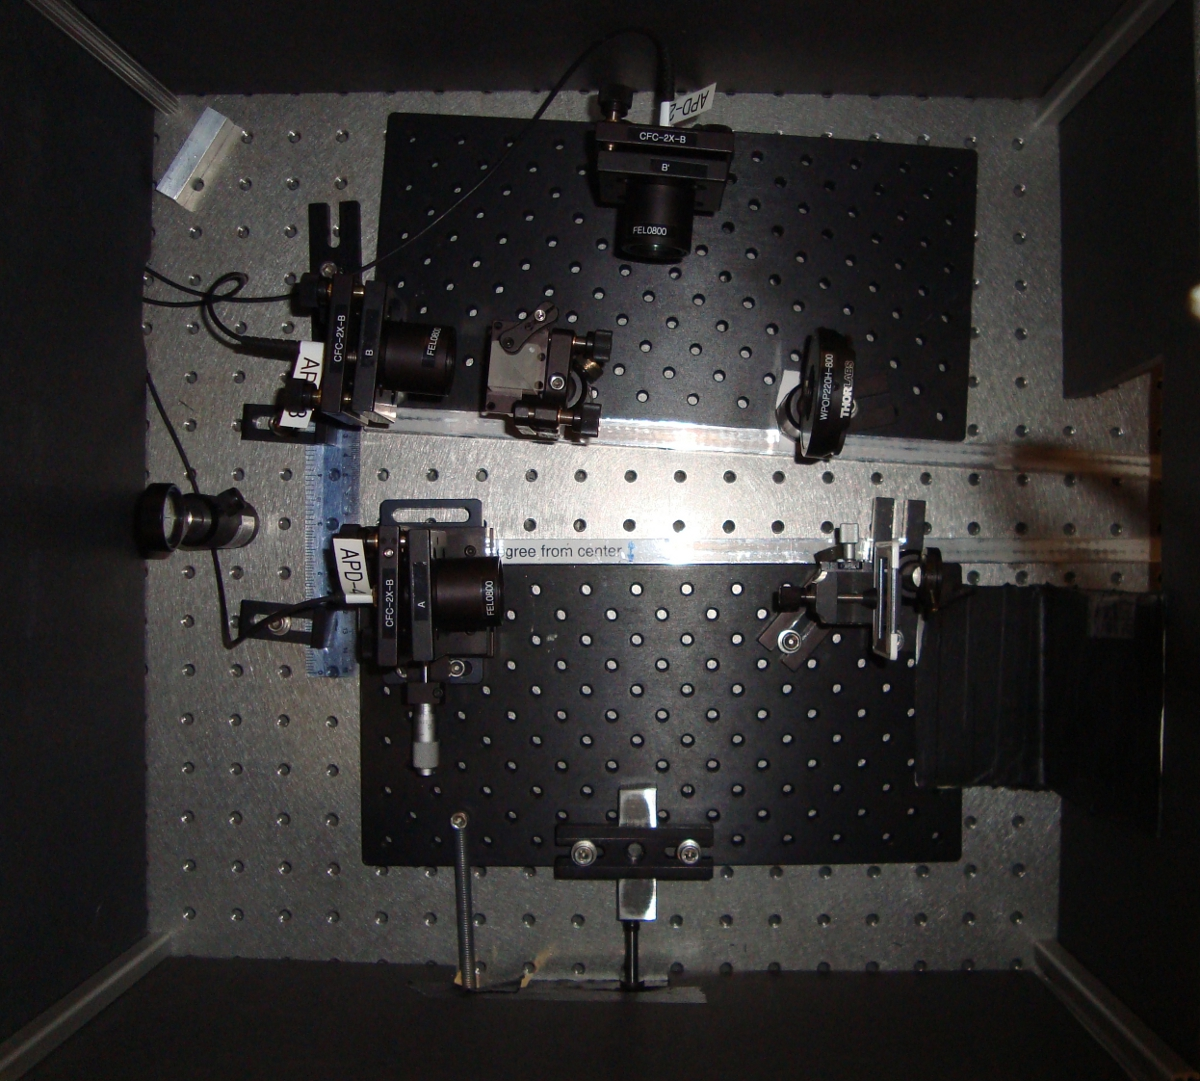
\includegraphics[width=0.25\linewidth,keepaspectratio]{images/Qe_overview.jpeg}}
\href{http://experimentationlab.berkeley.edu/sites/default/files/images/Qe_405interference.jpeg}{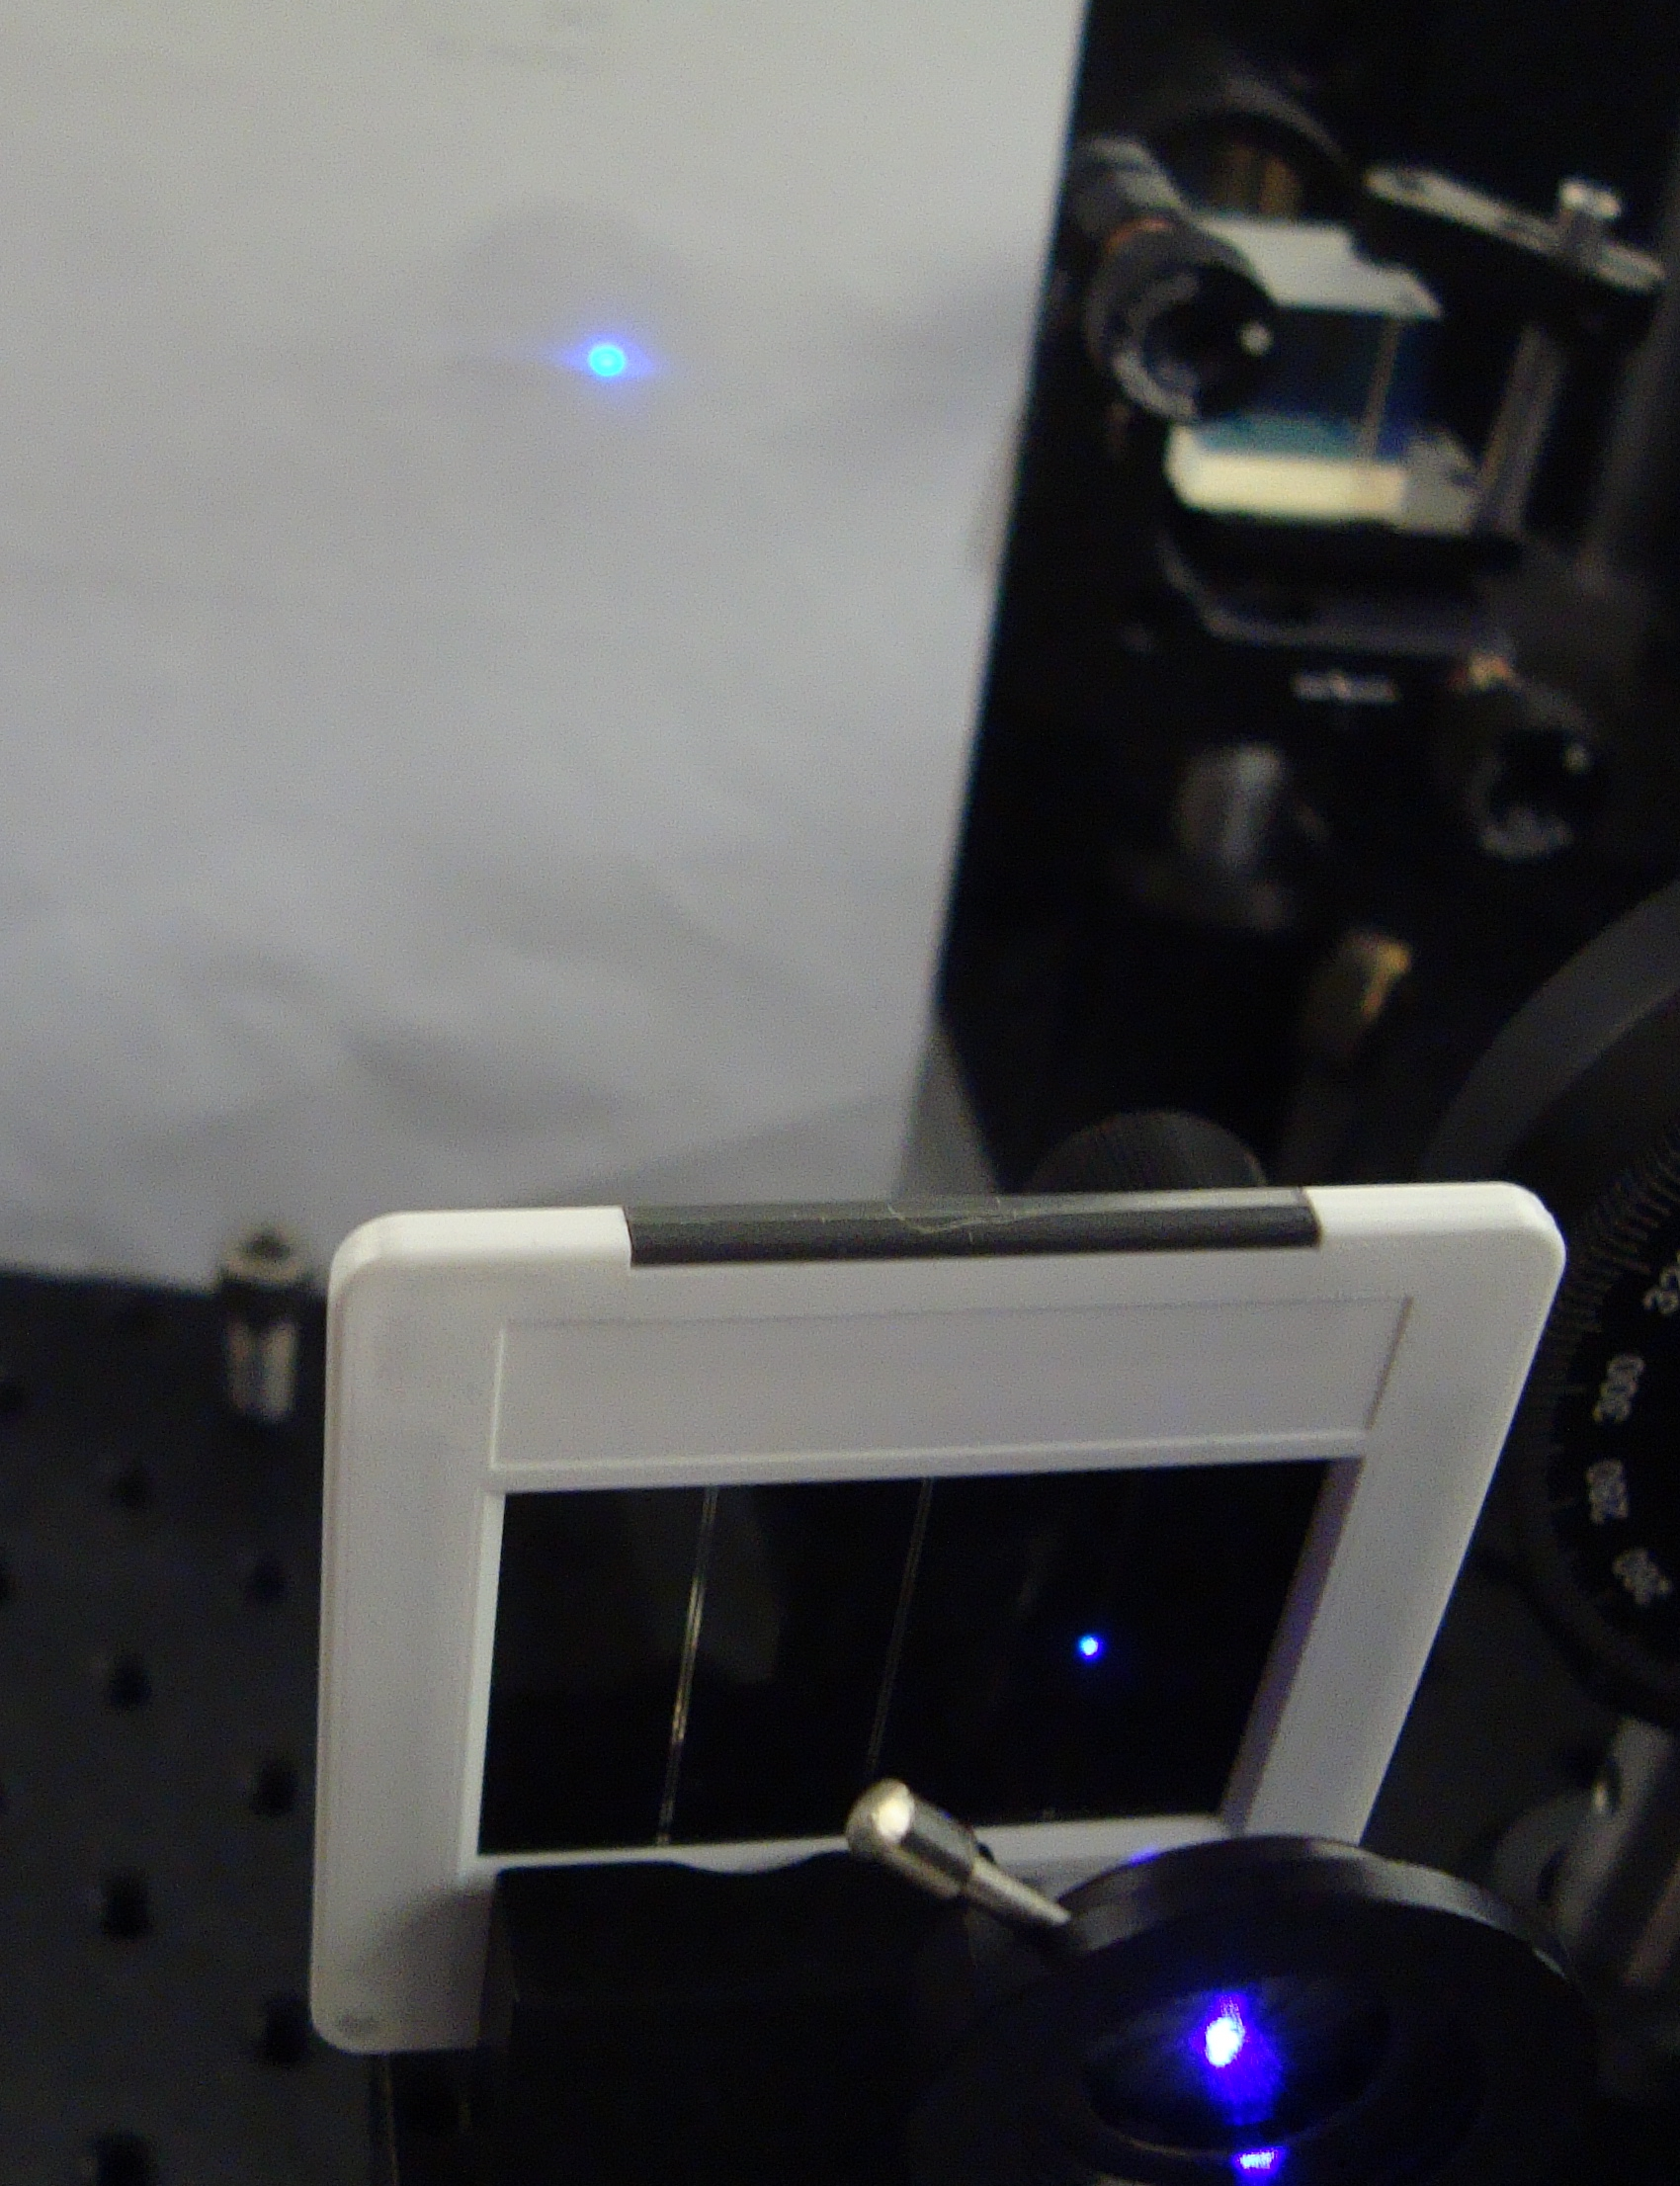
\includegraphics[width=0.25\linewidth,keepaspectratio]{images/Qe_405interference.jpeg}}
\href{http://experimentationlab.berkeley.edu/sites/default/files/images/Qe_beamview.jpeg}{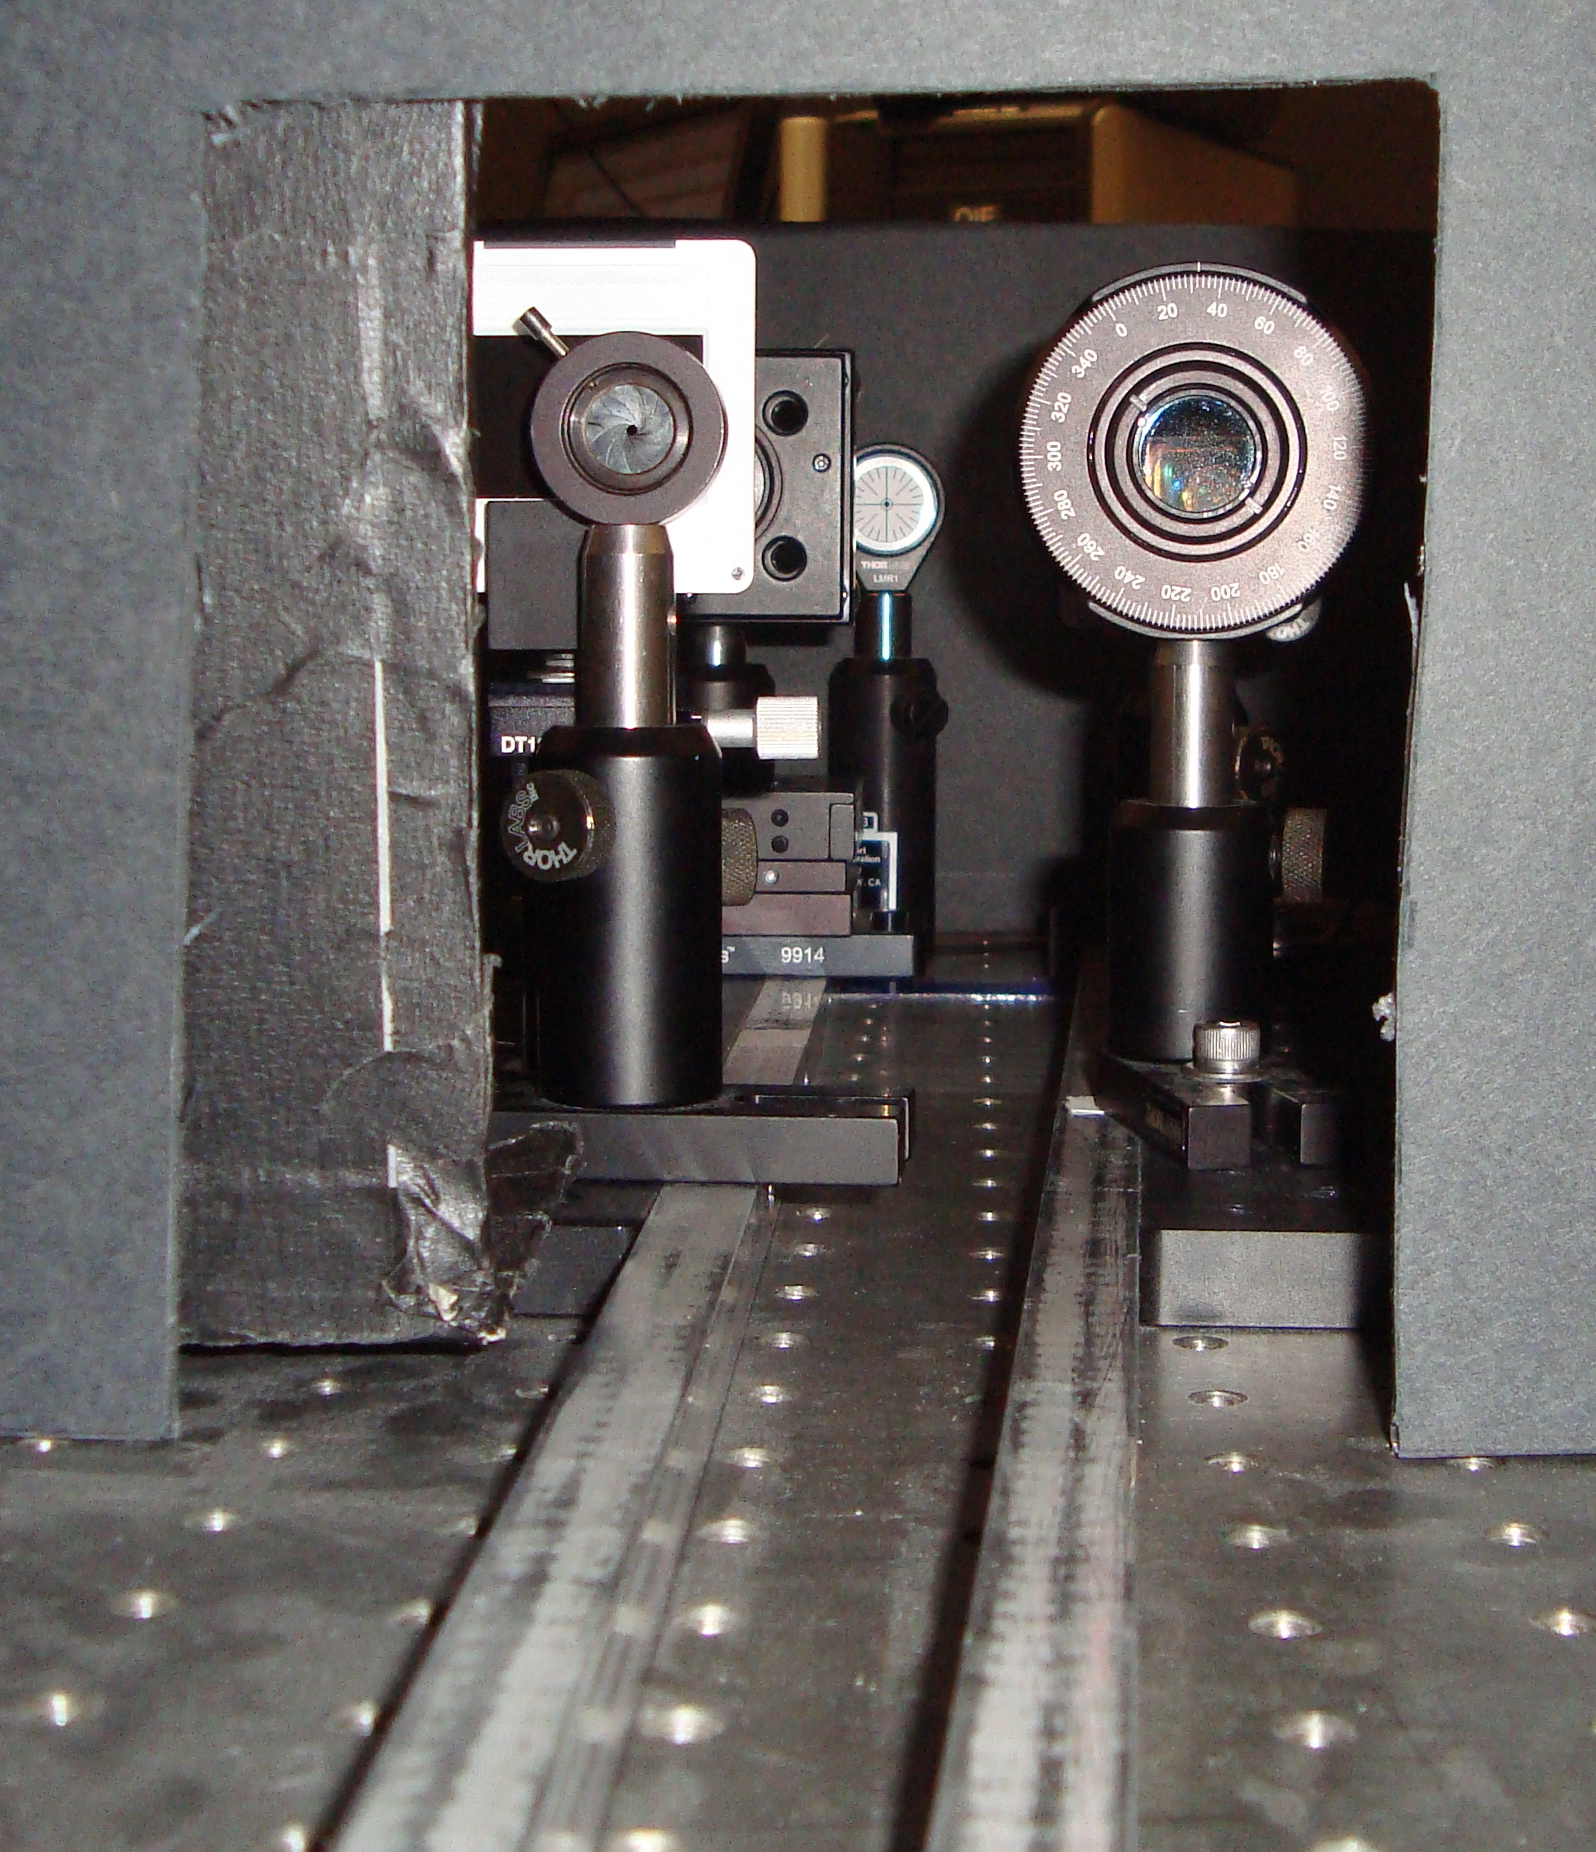
\includegraphics[width=0.25\linewidth,keepaspectratio]{images/Qe_beamview.jpeg}}
\href{http://experimentationlab.berkeley.edu/sites/default/files/images/Qe_slit.jpeg}{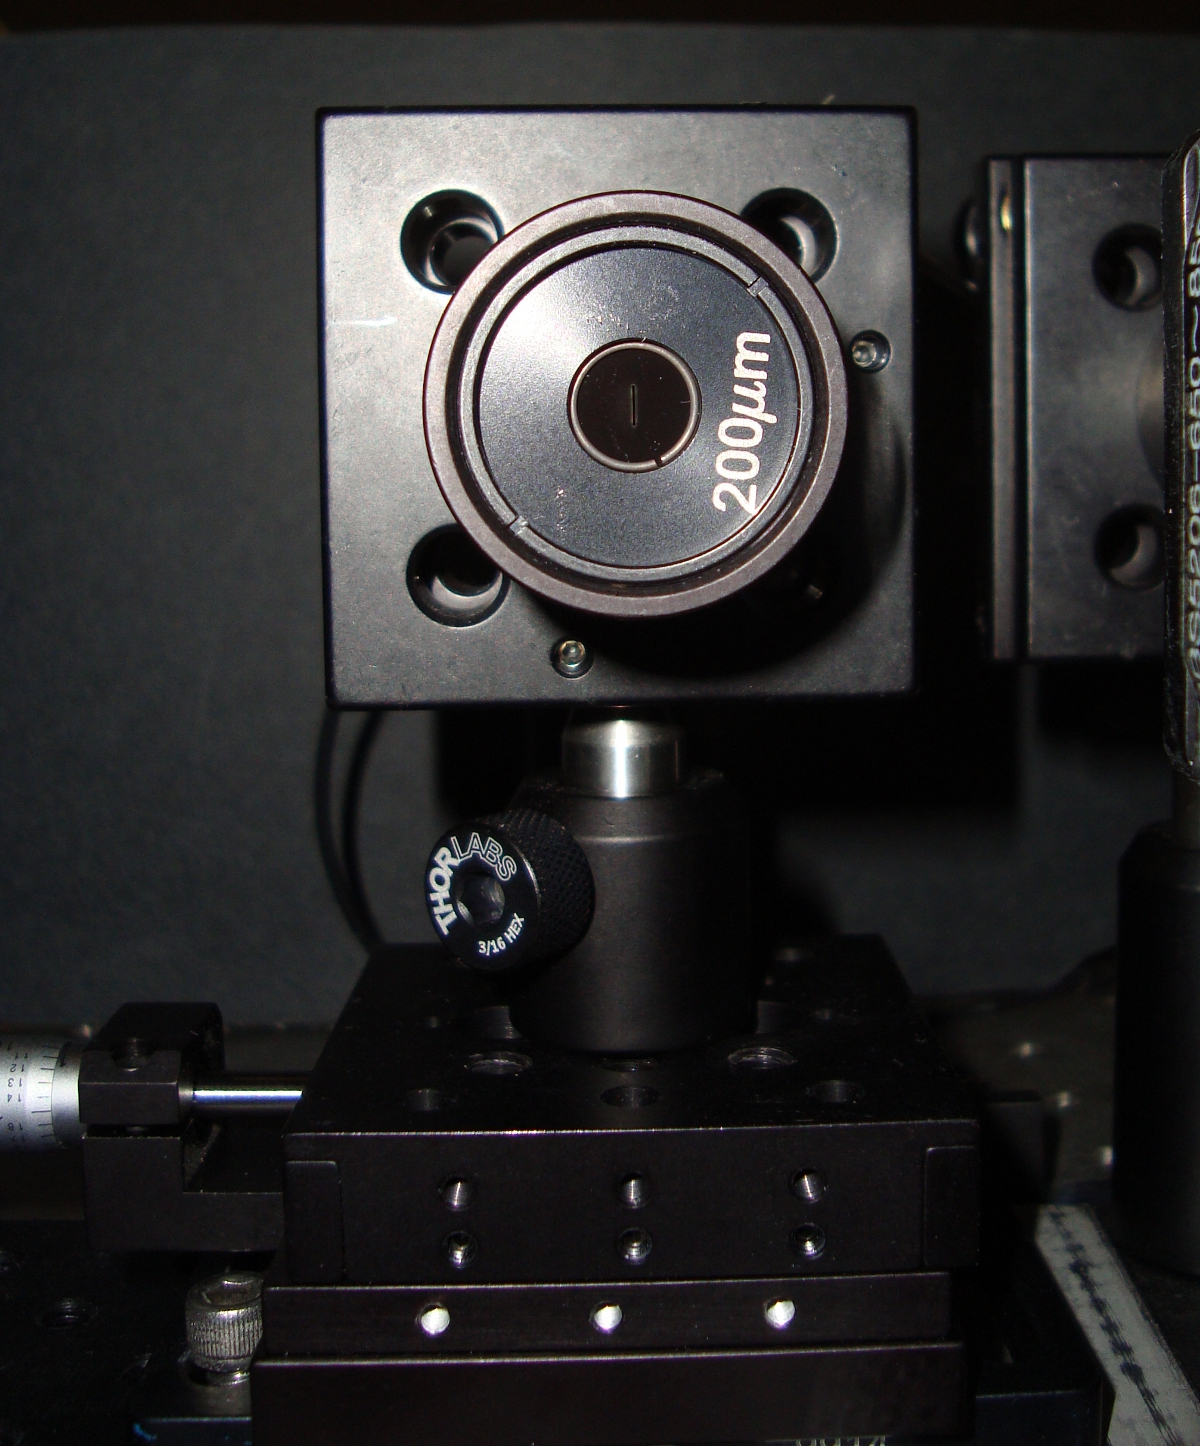
\includegraphics[width=0.25\linewidth,keepaspectratio]{images/Qe_slit.jpeg}}

\section{Trouble shooting}

Insufficient single photon counts in each detector (<10k/s)

\begin{enumerate}
    \item Is there enough blue laser power? You should have at least 35 mW (corresponds to about 50 mW at the laser diode) reasonably well collimated and focused after the BBOs before the band stop. If you decide to measure this power please consult the staff because there are safety concerns.

    \item Are the detectors properly aligned?

    \item Are the fibers inserted properly into their connectors? The image from the fiber tester at the BBO should be at most twice as large as the BBOs. If this is not the case most likely you have not inserted the fibers correctly into the detector port. Gently rotate the fiber till the notches on the fiber connector line up with the detector port and the connector slides into the port.
\end{enumerate}

\noindent Low or no coincidence counts (<200/s without polarization analysis):

\begin{enumerate}
    \item Is the half wave plate between the steering mirrors rotated by a reasonable angle? Angles > 45 degrees can distort the blue beam and thus limit the number of coincidences severely.
\end{enumerate}

\noindent Vastly different coincidence counts for vv and hh even though the blue polarization is set properly.

\begin{enumerate}
    \item Are the BBO's perpendicular to the violet light? You can adjust the downconversion efficiencies for the horizontal and the vertical beams independently by changing the angle of the BBO's with respect to the violet light. Why does this work?
\end{enumerate}

\noindent Coincidence rates as a function of the angle of the measurement basis make no sense

\begin{enumerate}
    \item Are you using halfwave plates for 800 nm or 400 nm to rotate the measurement basis?

    \item Do you really observe photon pair coincidences or are those accidental ones, i.e. the single-detector count-rates are too high?
\end{enumerate}

\begin{thebibliography}{}
\label{sec:References}
    \bibitem{Dehlinger} 
    \href{http://physics111.lib.berkeley.edu/Physics111/Reprints/QIE/Entangled\%20Photons-M.W.\%20Mitchell_1.1498860.pdf}{\textbf{1.1}} D. Dehlinger and M.W. Mitchell, ``Entangled photons, nonlocality, and Bell inequalities in the undergraduate laboratory''.

    \bibitem{Bell}
    J.S. Bell, \href{http://physics111.lib.berkeley.edu/Physics111/Reprints/QIE/Bell_Compact.pdf}{\textbf{``On the Einstein Podolsky Roden paradox''}}.

    \bibitem{Clauser}
    \href{http://prl.aps.org/abstract/PRL/v23/i15/p880/_1}{\textbf{3.1}} J.F. Clauser, M.A. Horne, A. Shimony and R.A. Holt, ``Proposed experiment to test local hidden-variable theories'', \href{http://prl.aps.org/abstract/PRL/v23/i15/p880/_1}{\textbf{Phys. Rev. Lett. 23, 880 (1969)}}.

    \bibitem{Walborn}
    S. P. Walborn, M. O. Terra Cunha, S. Pádua and C. H. Monken, ``Double-slit quantum eraser'', \href{http://physics111.lib.berkeley.edu/Physics111/Reprints/QIE/Quantum-Eraser-Walborn.pdf}{\textbf{Phys. Rev. A 65, 033818 (2002)}}.

    \bibitem{Fox}
    \href{http://site.ebrary.com/lib/berkeley/reader.action?ppg=40&docID=10177967&tm=1439419508236}{\textbf{Fox, Mark. Quantum Optics : An Introduction.}} Oxford, GBR: Oxford University Press, UK, 2006. ProQuest ebrary. Web. 12 August 2015. Search the index for ``Sum Frequency Mixing''

\end{thebibliography}

\vspace{1em}

\noindent Other reprints and reference materials can be found on the \href{\LabReprints}{\textbf{Physics 111 Library Site}}

\end{document}
